%%%%%%%%%%%%%%%%%%%%%%%%%%%%%%%%%%%%%%%%%
% Masters/Doctoral Thesis
% LaTeX Template
% Version 2.5 (27/8/17)
%
% This template was downloaded from:
% http://www.LaTeXTemplates.com
%
% Version 2.x major modifications by:
% Vel (vel@latextemplates.com)
%
% This template is based on a template by:
% Steve Gunn (http://users.ecs.soton.ac.uk/srg/softwaretools/document/templates/)
% Sunil Patel (http://www.sunilpatel.co.uk/thesis-template/)
%
% Template license:
% CC BY-NC-SA 3.0 (http://creativecommons.org/licenses/by-nc-sa/3.0/)
%
%%%%%%%%%%%%%%%%%%%%%%%%%%%%%%%%%%%%%%%%%


%----------------------------------------------------------------------------------------
%	PACKAGES AND OTHER DOCUMENT CONFIGURATIONS
%----------------------------------------------------------------------------------------

\documentclass[
11pt,                   % The default document font size, options: 10pt, 11pt, 12pt
%oneside,               % Two side (alternating margins) by default, uncomment to switch to one side
english,                % The language option
singlespacing,          % Single line spacing, alternatives: onehalfspacing or doublespacing
%draft,                 % Uncomment to enable draft mode (no pictures, no links, overfull hboxes indicated)
%nolistspacing,         % If the document is onehalfspacing or doublespacing, uncomment this to set spacing in lists to single
%liststotoc,            % Uncomment to add the list of figures/tables/etc to the table of contents
%toctotoc,              % Uncomment to add the main table of contents to the table of contents
%parskip,               % Uncomment to add space between paragraphs
%nohyperref,            % Uncomment to not load the hyperref package
headsepline,            % Uncomment to get a line under the header
%chapterinoneline,      % Uncomment to place the chapter title next to the number on one line
%consistentlayout,      % Uncomment to match to default the layout of the declaration, abstract...
]{MastersDoctoralThesis}

\usepackage[utf8]{inputenc}   % Required for inputting international characters
\usepackage[T1]{fontenc}      % Output font encoding for international characters
\usepackage{mathpazo}         % Use the Palatino font by default
\usepackage{mathtools}        % it also loads amsmath
\usepackage{amssymb}          % it also loads amsfonts
\usepackage{bm}               % bold Greek letters
\usepackage{xfrac}            % slanted frac
\usepackage{subcaption}       % sub-figures
\usepackage{fix-cm}           % arbitrary font size
\usepackage{float}            % placing figures
\usepackage{multirow}         % join cells at different rows of a table
\usepackage{makecell}         % makecell command, allow line break inside a cell of a table
\usepackage[backend=bibtex8,style=numeric-comp,giveninits=true,natbib=true,maxbibnames=9,maxcitenames=7]{biblatex}

\addbibresource{../bibliography/sw.bib}

\usepackage[autostyle=true]{csquotes} % Language-dependent quotes in the bibliography

%----------------------------------------------------------------------------------------
%	SECTIONING DEFINITIONS
%----------------------------------------------------------------------------------------

\setcounter{tocdepth}{3}
\setcounter{secnumdepth}{3}

%----------------------------------------------------------------------------------------
%	CUSTOM DEFINITIONS
%----------------------------------------------------------------------------------------

\newcommand{\pder}[2]{\frac{\partial#1}{\partial#2}}
\newcommand*{\ppder}[2]{\frac{\partial^2#1}{\partial#2^2}}
\newcommand*{\abs}[1]{\lvert#1\rvert}
\newcommand*{\norm}[1]{\lVert#1\rVert}
\newcommand*{\defeq}{\mathrel{\vcenter{\baselineskip0.5ex\lineskiplimit0pt\hbox{\scriptsize.}\hbox{\scriptsize.}}}=}
\newcommand*{\ldbrace}{\{\mskip-5mu\{} % left double curly braces
\newcommand*{\rdbrace}{\}\mskip-5mu\}} % right double curly braces


%----------------------------------------------------------------------------------------
%	MARGIN SETTINGS
%----------------------------------------------------------------------------------------

\geometry{
	paper=a4paper, % Change to letterpaper for US letter
	inner=2.5cm, % Inner margin
	outer=3.8cm, % Outer margin
	bindingoffset=.5cm, % Binding offset
	top=1.5cm, % Top margin
	bottom=1.5cm, % Bottom margin
	%showframe, % Uncomment to show how the type block is set on the page
}


%----------------------------------------------------------------------------------------
%	THESIS INFORMATION
%----------------------------------------------------------------------------------------

\date{July 1, 2022}
\thesistitle{Coupling shallow water models with three-dimensional models for the study of fluid-structure interaction problems using the particle finite element method} % print it with \ttitle
\supervisor{Dr. Eugenio \textsc{Oñate}} % print it with \supname
\cosupervisor{Dr. Ignasi \textsc{de-Pouplana}} % print it with \cosupname
\examiner{} % this is not currently used, print it with \examname
\degree{Civil Engineering Ph. D.} % print it with \degreename
\author{Miguel \textsc{Masó}} % print it with \authorname
\addresses{} % this is not currently used, print it with \addressname
\subject{Civil Engineering} % this is not currently used, print it with \subjectname
\keywords{} % this is not currently used, print it with \keywordnames
\university{\href{http://www.upc.edu}{Universitat Politècnica de Catalunya Barcelona Tech}} % print it with \univname
\department{\href{http://www.deca.upc.edu}{Department of Civil and Environmental Engineering}} % print it with \deptname
\group{\href{http://www.cimne.com}{International Centre for Numerical Methods in Engineering}} % print it with \groupname
\faculty{\href{http://www.etseccpb.upc.edu}{Barcelona School of Civil Engineering}} % print it with \facname

\colorlet{wrmBlue}{blue!30!black}
\colorlet{wrmGreen}{green!30!black}
\AtBeginDocument{
\hypersetup{pdftitle=\ttitle} % Set the PDF's title to your title
\hypersetup{pdfauthor=\authorname} % Set the PDF's author to your name
\hypersetup{pdfkeywords=\keywordnames} % Set the PDF's keywords to your keywords
\hypersetup{linkcolor=wrmBlue}
\hypersetup{citecolor=wrmGreen}
}



%%%%%%%%%%%%%%%%%%%%%%%%%%%%%%%%%%%%%%%%%%%%%%%%%%%%%%%%%%%%%%%%%%%%%%%%%%%%%%%%%%%%%%%%%
%%%%%%%%%%%%%%%%%%%%%%%%%%%%%%%%%%%%%%%%%%%%%%%%%%%%%%%%%%%%%%%%%%%%%%%%%%%%%%%%%%%%%%%%%
%%%%%%%%%%%%%%%%%%%%%%%%%%%%%%%%%%%%%%%%%%%%%%%%%%%%%%%%%%%%%%%%%%%%%%%%%%%%%%%%%%%%%%%%%

% \includeonly{chapters/equations, chapters/eulerian_sw, chapters/eulerian_bsq}

%%%%%%%%%%%%%%%%%%%%%%%%%%%%%%%%%%%%%%%%%%%%%%%%%%%%%%%%%%%%%%%%%%%%%%%%%%%%%%%%%%%%%%%%%
%%%%%%%%%%%%%%%%%%%%%%%%%%%%%%%%%%%%%%%%%%%%%%%%%%%%%%%%%%%%%%%%%%%%%%%%%%%%%%%%%%%%%%%%%
%%%%%%%%%%%%%%%%%%%%%%%%%%%%%%%%%%%%%%%%%%%%%%%%%%%%%%%%%%%%%%%%%%%%%%%%%%%%%%%%%%%%%%%%%



\begin{document}

\frontmatter % Use roman page numbering style (i, ii, iii, iv...) for the pre-content pages

\pagestyle{plain} % Default to the plain heading style until the thesis style is called for the body content


%----------------------------------------------------------------------------------------
%	TITLE PAGE
%----------------------------------------------------------------------------------------

\begin{titlepage}
\begin{center}

\vspace*{.06\textheight}
{\scshape\LARGE \univname\par}\vspace{1.5cm} % University name
\textsc{\Large Doctoral Thesis}\\[0.5cm] % Thesis type

\HRule \\[0.4cm] % Horizontal line
{\huge \bfseries \ttitle\par}\vspace{0.4cm} % Thesis title
\HRule \\[1.5cm] % Horizontal line
 
\begin{minipage}[t]{0.4\textwidth}
\begin{flushleft} \large
\emph{Author:}\\
\href{https://directori.upc.edu/directori/dadesPersona.jsp?id=1115243}{\authorname}
\end{flushleft}
\end{minipage}
\begin{minipage}[t]{0.4\textwidth}
\begin{flushright} \large
\emph{Supervisors:} \\
\href{http://www.cimne.com/eo}{\supname} \\
\href{https://www.cimne.com/1898/2181/people/directory}{\cosupname}
\end{flushright}
\end{minipage}\\[.3cm]
 
\vfill

\large \textit{A thesis submitted in fulfillment of the requirements\\ for the degree of \degreename}\\[0.3cm] % University requirement text
\textit{in the}\\[0.3cm]
\groupname\\\deptname\\[.3cm] % Research group name and department name
 
\vfill

{\large \printdate}\\[1cm]
\href{https://camins.upc.edu/}{
\includegraphics[width=.6\textwidth]{img/logo_caminos.png}
}
\vfill
\end{center}
\end{titlepage}


%----------------------------------------------------------------------------------------
%	DECLARATION PAGE
%----------------------------------------------------------------------------------------

% \begin{declaration}
% \addchaptertocentry{\authorshipname} % Add the declaration to the table of contents
% \noindent I, \authorname, declare that this thesis titled, \enquote{\ttitle} and the work presented in it are my own. I confirm that:

% \begin{itemize} 
% \item This work was done wholly or mainly while in candidature for a research degree at this University.
% \item Where any part of this thesis has previously been submitted for a degree or any other qualification at this University or any other institution, this has been clearly stated.
% \item Where I have consulted the published work of others, this is always clearly attributed.
% \item Where I have quoted from the work of others, the source is always given. With the exception of such quotations, this thesis is entirely my own work.
% \item I have acknowledged all main sources of help.
% \item Where the thesis is based on work done by myself jointly with others, I have made clear exactly what was done by others and what I have contributed myself.\\
% \end{itemize}
 
% \noindent Signed:\\
% \rule[0.5em]{25em}{0.5pt} % This prints a line for the signature
 
% \noindent Date:\\
% \rule[0.5em]{25em}{0.5pt} % This prints a line to write the date
% \end{declaration}

% \cleardoublepage


%----------------------------------------------------------------------------------------
%	QUOTATION PAGE
%----------------------------------------------------------------------------------------

% \vspace*{0.2\textheight}
% \noindent\enquote{\itshape And besides these, be warned – the making of many books has no end, and much study is a wearying of the flesh.}\bigbreak
% \hfill Qo 12, 12


%----------------------------------------------------------------------------------------
%	ABSTRACT PAGE
%----------------------------------------------------------------------------------------

\begin{abstract}
This thesis investigates numerical methods for the simulation of surface water flows, focusing on the interaction between the large scale and the local scale and its application to natural hazards. Several families of numerical methods for the approximation of large scale phenomena and the coupling with the local scale have been analyzed.

The general motion of a fluid mass is governed by the Navier-Stokes equations, which can accurately solve the local scale phenomena. However, the same level of accuracy is not required by the large scale solution of the water-related events. In this context, the shallow water equations are defined. In contrast to the extensive use of the Finite Element Method for solving the Navier-Stokes equations, the shallow-water equations are usually solved with the Finite Volume Method. Thus, an effort have been done to solve both equations in an unified framework.

The first part of this thesis is devoted to study stabilized formulations of Finite Element Method for the different forms of the shallow water equations. Stabilized formulations arise from the need to mitigate the various instabilities inherent in numerical approximations. The first source of instability is the incompatibility of the equal interpolation of the variables. The second source of instability is the presence of shocks due to the change of regime or hydraulic jumps. Finally, Gibbs oscillations may appear on the moving shoreline and monotonic properties of the physical system are lost by the numerical approximation.

The second part of the thesis is committed to the coupling strategies of the numerical methods for the Navier-Stokes and the shallow water equations. The case of a coupling from the local scale to the large scale is analyzed. This type of coupling corresponds to the generation of cascading natural hazard. The proposed strategy combines a Lagrangian Navier Stokes multi-fluid solver with an Eulerian method based on the Boussinesq equations, an extension of the shallow water equations.

Finally, the proposed technique is applied to the numerical simulation of landslide-generated impulse waves. The Particle Finite Element Method has been used to model the landslide runout, its impact against the water body and the consequent wave generation. The results of this fully-resolved analysis are stored at selected interfaces and then used as input for the modelling of waves propagation on the far-field.
This one-way coupling scheme drastically reduces the computational cost of the analyses while maintaining high accuracy in reproducing the key phenomena of cascading natural hazards.
\end{abstract}


%----------------------------------------------------------------------------------------
%	ABSTRACT PAGE
%----------------------------------------------------------------------------------------

\begin{resumen}
En esta tesis se investigan métodos numéricos para la simulación de flujos de aguas superficiales, haciendo énfasis en la interacción entre las distintas escalas y su aplicación a desastres naturales. Se han analizado diversas familias de métodos numéricos para aproximar los fenómenos a gran escala y su acoplamiento con la escala local.

El movimiento general de una masa de fluido se rige por las ecuaciones de Navier-Stokes, que pueden resolver con precisión los fenómenos a escala local. Sin embargo, la solución numérica a gran escala de dichos fenómenos, no requiere el mismo nivel de precisión. En este ámbito, se definen las acuaciones de agua poco profundas. En contraste con el amplio uso del Método de los Elementos Finitos para aproximar las ecuaciones de Navier-Stokes, las ecuaciones de aguas poco profundas se suelen resolver con el Método de los Volúmenes Finitos. Por ello, se ha realizado un esfuerzo para resolver ambas ecuaciones en un marco unificado.

La primera parte de esta tesis está dedicada a estudiar formulaciones estabilizadas para el Método de los Elementos Finitos aplicado a las diferentes formas de las ecuaciones de aguas someras. Las formulaciones estabilizadas surgen de la necesidad de mitigar las diferentes inestabilidades inherentes a las aproximaciones numéricas. La primera fuente de inestabilidad es la incompatibilidad debida a la interpolación de las variables. La segunda fuente de inestabilidad es la presencia de discontinuidades debidos al cambio de régimen o a los saltos hidráulicos. Por último, pueden aparecer oscilaciones de Gibbs en la línea de costa en movimiento, dado que las propiedades monótonas del sistema físico se pierden por la aproximación numérica.

La segunda parte de la tesis está dedicada a las estrategias de acoplamiento de los métodos numéricos para las ecuaciones de Navier-Stokes y de aguas poco profundas. Se ha analizado el caso de acoplamiento desde la escala local a la escala global. Este tipo de acoplamiento corresponde a la generación de desastres naturales en cascada. La estrategia propuesta combina un solver Lagrangiano de Navier Stokes para multi-fluidos con un método Euleriano basado en las ecuaciones de Boussinesq, una extensión de las ecuaciones de aguas someras.

Finalmente, la técnica propuesta se ha aplicado a la simulación numérica de olas generadas por deslizamientos. El deslizamiento de ladera, su impacto contra la masa de agua y la consiguiente generación de olas se ha modelado con el Método de Elementos Finitios de Partículas. Los resultados de este análisis detallado se almacenan en las interfaces seleccionadas que, luego, se utilizan como punto de entrada para modelar la propagación de olas en el campo lejano.
Este esquema de acoplamiento unidireccional reduce drásticamente el coste computacional, a la vez que se mantiene una alta precisión en la simulación de los fenómenos clave de desastres naturales.
\end{resumen}


%----------------------------------------------------------------------------------------
%	ACKNOWLEDGEMENTS
%----------------------------------------------------------------------------------------

\begin{acknowledgements}
Over the years developing this thesis there have been many people around me who have helped me to achieve this goal. 
I am indebted to all of them and it would be impossible to mention all of them.

I want to thank to Jaume Armenogu, who encouraged me to begin a Doctorate, and also to thank Eugenio Oñate for giving me the opportunity to work on this thesis and for his advices as supervisor. I also want to thank Ignasi de-Pouplana for being my co-supervisor.

From CIMNE, tanks to Sergio Idelsohn and Riccardo Rossi for all the clarifying and fruitful lessons that they have given to me. Thanks to Alessando and Alejandro for their collaboration during the last part of the thesis. I also want to mention my colleagues who finished their doctorate in the previous years and I have been helped by their knowledge and advice, Vicente, Pablo, Jordi, Guillermo, Rubén. Let me also mention my colleagues from CIMNE. From CIMAT, thanks to Prof. Botello, Jorge López and all the friends I met in Guanajuato.

In the same line, thanks to all my colleagues, friends and so many other people that I may
not mention explicitly. Thanks to my family for their constant support and encouragement.

Finally, I want to acknowledge the doctoral scholarship received from Universitat Politècnica de Catalunya and Banco Santander (53 FPI-UPC 2018) and the big support that CIMNE gave to this research.
\end{acknowledgements}


%----------------------------------------------------------------------------------------
%	LIST OF CONTENTS/FIGURES/TABLES PAGES
%----------------------------------------------------------------------------------------

\tableofcontents % Prints the main table of contents

\listoffigures % Prints the list of figures

\listoftables % Prints the list of tables


%----------------------------------------------------------------------------------------
%	ABBREVIATIONS
%----------------------------------------------------------------------------------------

\begin{abbreviations}{ll}
% Include a list of abbreviations (a table of two columns)
ALE   & Arbitrary Lagrangian Eulerian \\
ASGS  & Algebraic Sub-Grid Scale \\
BDF   & Backward Differentiation Formula \\
CG    & Continuous Galerkin \\
DG    & Discontinuous Galerkin \\
DAB   & Double Absorbing Layer \\
FC    & Flux Correction \\
FD    & Finite Difference method \\
FEM   & Finite Element Method \\
FFS   & Far-Field Solver \\
FIC   & Finite-Increment Calculus \\
FSI   & Fluid-Structure Interaction \\
FV    & Finite Volume method \\
GJV   & Gradient Jump viscosity \\
LGW   & Landslide Generated Wave \\
LTS   & Local Time Step \\
MPM   & Material Point Method \\
NFS   & Near-Field Solver \\
NS    & Navier-Stokes \\
PFEM  & Particle Finite Element Method \\
PFEM2 & Particle Finite Element Method 2-nd generation \\
PML   & Perfectly Matched Layer \\
RV    & Residual Viscosity \\
SPH   & Smooth Particle Hydrodynamics \\
SUPG  & Stream-Upwind Petrov-Galerkin \\
SW    & Shallow Water \\
TVD   & Total Variational Diminishing \\
VMS   & Virtual Multi-Scale \\
VOF   & Volume Of Fluid \\
\end{abbreviations}


%----------------------------------------------------------------------------------------
%	PHYSICAL CONSTANTS/OTHER DEFINITIONS
%----------------------------------------------------------------------------------------

% \begin{constants}{lr@{${}={}$}l}
% % The \SI{}{} command is provided by the siunitx package
% % The list of physical constants is a three column table
% % Constant Name & $Symbol$ & $Constant Value$ with units\\
% Gravity          & $g$     & \SI{9.81}{\meter\per\square\second} \\
% Water density    & $\rho$  & \SI{1000}{\kilo\gram\per\cubic\metre} \\
% Water viscosity  & $\nu$   & \SI{1.0}{\milli\pascal\second} (at \SI{20}{\celsius}) \\
% \end{constants}


%----------------------------------------------------------------------------------------
%	SYMBOLS
%----------------------------------------------------------------------------------------

% \begin{symbols}{lll}
% % Include a list of Symbols (a three column table)
% % Symbol & Name & Unit \\
% $g$       & Gravity           & \si{\meter\per\square\second} \\
% $\rho$    & Density           & \si{\kilo\gram\per\cubic\metre} \\
% $\nu$     & Viscosity         & \si{\milli\pascal\second} \\

% \addlinespace % Gap to separate the Roman symbols from the Greek

% $\omega$ & angular frequency & \si{\radian} \\

% \end{symbols}


%----------------------------------------------------------------------------------------
%	DEDICATION
%----------------------------------------------------------------------------------------

% \dedicatory{For/Dedicated to/To my\ldots} 


%----------------------------------------------------------------------------------------
%	THESIS CONTENT - CHAPTERS
%----------------------------------------------------------------------------------------

\mainmatter % Begin numeric (1,2,3...) page numbering

\pagestyle{thesis} % Return the page headers back to the "thesis" style


\chapter{Introduction}
\label{chapter_introduction}

Floods are complex natural phenomena with a great assortment of causes and a huge casuistic
depending on the land characteristics or the climatic conditions. Preventing floods is still a great
challenge due to uncertainty of climatic conditions and complexity of modeling land, usually
defined by a great number of variables and parameters.
Some of the main flooding causes are torrential storms, hurricanes or monsoon, reservoir failure
or small floodplains. Near coastal zones floods are also caused by storm surges or even
tsunami waves. In the case of lakes and reservoirs, long waves may be generated by landslides.

Flooding is the most important natural hazard in terms causing of loss of life, displacement of
people and economic losses. But vulnerability can
increase when natural hazards make strategic structures fail, or when there aren't precautionary
measures or actuation plans.



Even thoug this study is about the numercial modelling of water related hazards and special attention has been paid to hydrological problems, the equations can be applied to a huge variety of problems. The configuration is modifyed just specifying the appropriate boundary conditions. Aside from the main scope of the thesis, some other examples are included. One example of application is related to pollutant transport in atmospheric environment. The other example is about tune liquid dampers for high rise buildings.



\section{Objectives} 

The main objective of this thesis is the coupling of different scales in natural hazards. Usually, the action is originated in a far filed from where the the vulnerability is located. There are three scenarios with different scale. The action may be generated in a local or global scale, depending on the nature of the phenomena. The propagation is usually in the large scale and it introduces the need of using reduced models. Finally, the evaluation of the resilience of singular structures requires to descend to the local scale.

The objectives can be sumarized as
\begin{itemize}
    \item aaa
\end{itemize}

Gran escala: simplificaciones 2D a las ecuaciones de Navier-Stokes.

Escala local: fenómenos turbulentos que requieren la solución de las ecuaciones de Navier-Stokes en 3D con alta resolución.


\section{State of the art}




\chapter{Free surface flows}


\section{Navier-Stokes equations}


\section{Shallow water equations}


\section{Boussinesq modified equations}




\chapter{Finite Element Methods for the shallow water equations}
\label{eulerian_sw}


Due to the complexity of the geometry and the source terms is not possible to find an analytical solution for the SW equations, this explains the need to design strategies to find numerical solutions. In this chapter some numerical strategies with the FEM in an eulerian framework are explored.
The Eulerian frameworks are robust and very efficient for continuous problems. However, discontinuities and front tracking may require especial attention. Since in those physical phenomena flooding or moving shoreline may occur, the identification of the dry domain is a challenging problem for the Eulerian FEM.
Moreover, monotonic properties are especially interesting when partially wet domains are considered, since the water depth is a positive magnitude but, in general, numerical methods does not verify this property.

The SW equations have traditionally been modelled using finite volumes (FV) because of its advantages of stability and monotonicity. Given its geometric flexibility and its natural way to introduce high order schemes, the FEM has been applied too \cite{zien3,navon1979,navon1988}.
Halfway between FV and FEM, there is the discontinuous Galerkin (DG) technique \cite{ambati2007,khan2014,lee2019}. DG method has the advantages of the geometrical flexibility of the FEM and the stability of FV, but the introduction of high order DG schemes is not straightforward.
Since the FEM can exhibit spurious oscillations, different strategies such as stabilization, monotonic schemes or different order of polynomial interpolation can be explored \cite{hood1974,zien3,ortiz2012}.




%This research is focused in classical stabilized finite elements with an equal order interpolation for all the variables. We will explore the capabilities of the finite increment calculus (FIC) technique to develop stable formulations for the SW equations.

In this chapter, the general procedure for FEM is presented. Then, some stabilization techniques are explored: the FIC-based stabilization, the flux corrected technique and the gradient jump viscosity method. Finally, the stabilized formulation is applied to the Boussinesq modified equations. Several examples are provided to show the capabilities and limitations of each method.




\section{Galerkin weak formulation}



We consider a balance equation in the space domain $\Omega$ and the time interval $[0,T]$. Let $\bm{\phi}$ and $\bm{\psi}$ be vector functions of the domain $\Omega \times [0,T]$ and $\mathbf{r}$ the residual of the balance equations expressed in terms of the unknown $\bm{\phi}$.
The space of functions that are square-integrable in $\Omega$ is denoted as $L^2(\Omega)$. And the space of functions whose derivatives up to order $m\geq0$ belong to $L^2(\Omega)$ is denoted by $H^m(\omega)$. The space $H_0^1(\Omega)$ consists on a subspace of $H^1(\Omega)$ vanishing on $\partial \Omega$.

Using this notation, the space of functions for the continuous problem are $V \defeq H^1(\Omega)$ and for the test functions $V_0 \defeq H_0^1(\Omega)$.
The variational form of the balance equations can be expressed as find $\bm{\phi} \in V$ such that $\forall \bm{\psi} \in V_0$
\begin{equation} \label{variational_form}
    \int_\Omega \bm{\psi} \cdot \mathbf{r}(\bm{\phi}) \ d\Omega = 0
\end{equation}



The standard Galerkin approximation \ref{variational_form} is straightforward. Let $\mathcal{P}_h$ be a partition of the domain $\Omega$. The diameter of an element domain $e\in\mathcal{P}_h$ is denoted by $l_e$. From the polynomial spaces defined by the finite elements, we can construct the subspaces $V_h\in V$ and $V_{h,0}\in V_0$. The Galerkin approximation of the balance equations can be expressed as find $\bm{\phi}_h \in V_h$ such that $\forall \bm{\psi} \in V_{h,0}$
\begin{equation} \label{discrete_variational}
    \int_\Omega \bm{\psi} \cdot \mathbf{r}(\bm{\phi}) \ d\Omega = 0
\end{equation}

Unfortunately, this problem is not straightforward to solve using finite elements, as its discrete version is not numerically stable. In fact, to ensure that the problem of finding $\bm{\phi}$ has a stable solution, the space must verify the inf-sub condition \cite{codina2011}.



\section{Stabilized formulations for the shallow water equations}


Several families of stabilization methods can be found in the literature, usually applied to the convection-diffusion equations and the Navier-Stokes equations. The most relevant are SUPG \cite{brooks1982},
ASGS\cite{codina1998}, GLS \cite{hughes1989} and FIC\cite{onate1996,onate1998}.
Due to the hyperbolic character of the SW equations, a particular stabilization method for compressible flow or the Euler equations need to be developed.
The FIC approach is based on the incremental solution of a modified system of non-local governing equations accounting for higher order terms obtained by applying the balance laws in domains of finite size.
The FIC-based stabilization has been applied in conjunction with the FEM to convection-diffusion, incompressible flows, among other applications \cite{onate1998,onate2001}.
In those cases, where the convective term has an important role, a first order FIC term is enough to provide stability to the system.
However, the SW equations are governed by the convective term and the wave equation in a mixed formulation \cite{codina2008}. In consequence, the common derivation of the FIC-based stabilization is not enough to provide stability in all the range of applicability of the SW equations. 
A generalization of this method is proposed in order to provide a global stability for the SW equations.

Once global stability is achieved, local instabilities may appear near discontinuities, which are inherent to the supercritical flows.
A local shock capturing technique was initially proposed by Hughes \cite{hughes1986} and a review of shock capturing techniques can be found in Codina \cite{codina2011}.
Other possibilities of the FIC-based formulations are explored to provide a shock capturing stabilization \cite{cotela2016}.

Additionally, the dry domain requires an accurate modeling because the hyperbolic equations require positive water depth in all the domain.
Several authors have proposed different methods to solve the shallow water equations with moving shoreline. Leclerc et al. \cite{leclerc1990} proposed an Eulerian method. Later, Heniche et al. \cite{heniche2000} modified the method allowing the free surface to plunge under the topography.
Other authors developed a rough-porous layer \cite{candy2017,barros2011} or a modified depth integration \cite{defina2000}. These approaches introduce new physical parameters in the balance equations.
An Eulerian approach based on the work of \cite{leclerc1990} and \cite{heniche2000} is presented.




\subsection{FIC stabilization}
\label{sec:stabilization}

We will consider the quasi-linear balance equations written in residual form as a vector

\begin{equation} \label{residual}
\mathbf{r} \defeq 
  \pder{\bm{\phi}}{t} + \mathbf{A}_i\pder{\bm{\phi}}{x_i}
  -\pder{}{x_i}\left(\mathbf{K}_{ij}\pder{\bm{\phi}}{x_j}\right) + \mathbf{S}\bm{\phi} + \mathbf{b}_i\pder{z}{x_i} \qquad i,k\in\{1,n_d\}
\end{equation}
where $n_d=2$ is the number of dimensions. The size of the vector $\mathbf{r}$ is equal to the number of balance equations, $n_b=3$.

In the one dimensional case ($n_d=1$) and scalar balance ($n_b=1$), the FIC-based stabilization is based on a modified non local version of the governing equations as \cite{onate1998}

\begin{equation}
r - \frac{1}{2}l^e\pder{r}{x} = 0
\end{equation}

The stabilization parameter $l^e$ is usually taken the element length. However, in 2D and 3D, or when the number of balance equations $n_b$ is different than $n_d$, the choice of the $l^e$ parameter is non trivial.
Several approaches can be found in the literature. In \cite{onate1998} $l^e$ is chosen as a vector, but in later publications such as \cite{onate2001} a generalized formulation for different values of $n_d$ and $n_b$ was presented.
For the stabilization of the Navier-Stokes equations different projections of the element size over the velocity and over the velocity gradient have been proposed \cite{cotela2016}. Here we will use index notation for the residual vector $\mathbf{r}$ in order to distinguish the indices that goes to $n_d$ or to $n_b$. To sum up, the different forms of the FIC stabilization procedure can be written as

\begin{subequations}
\begin{align}
r_{k} - \frac{1}{2}l^e_i\pder{r_k}{x_i} &= 0
    \qquad i\in\{1,n_d\} \ ,\ k\in\{1,n_b\}\\[5pt]
r_{k} - \frac{1}{2}l^e_u\frac{u_i}{\norm{\mathbf{u}}}\pder{r_k}{x_i} &= 0
    \qquad i,k\in\{1,n_d\}\\[5pt]
r_{k} - \frac{1}{2}l^e_{g_i}\frac{\sfrac{\partial\mathbf{u}}{\partial x_i}}{\norm{\nabla u_i}}\pder{r_k}{x_i} &= 0
    \qquad i,k\in\{1,n_d\}
\end{align}
\end{subequations}

We propose a stabilization term which is oriented along the characteristics of the hyperbolic equations, as

\begin{equation} \label{fic_sw}
r_{k} - \frac{1}{2}l^e\frac{\mathbf{A}_i}{\lambda}\pder{r_k}{x_i} = 0
    \qquad i\in\{1,n_d\} \ ,\ k\in\{1,n_b\}
\end{equation}
For consistency the linearization matrix $\mathbf{A}_i$ is normalized with the maximum eigenvalue $\lambda=\abs{\mathbf{u}} + c$. This stabilization is analogue to the virtual multi-scale stabilization proposed in \cite{codina2008b}. The linearization matrix $\mathbf{A}_i$ provides a weighting procedure between the stabilization of the convective and the mixed wave equation terms. In practice the element size is multiplied by an algorithmic constant in order to control the amount of diffusion added by the stabilization and it will be studied in the examples of Section \ref{sec:examples}. Recovering the vector notation for the residual, the FIC-balance reads
\begin{equation} \label{fic_sw_beta}
\mathbf{r} - \beta l^e\frac{\mathbf{A}_i}{\lambda}\pder{\mathbf{r}}{x_i}
    \qquad i\in\{1,n_d\}
\end{equation}

The FIC formulation is the result of introducing the residual of the shallow water equations (\ref{residual}) into the expression in Eq (\ref{fic_sw_beta}). The variational expression of the equation is obtained by multiplying the equation by a test function $\omega_k$ and integrating over the domain $\Omega$. This gives

\begin{equation} \label{variational_fic}
\int_\Omega \left(
    \omega_k \mathbf{r} - \omega_k \beta l^e\frac{\mathbf{A}_i}{\lambda}\pder{\mathbf{r}}{x_i}
\right) d\Omega = 0
\end{equation}
The second term of Equation (\ref{variational_fic}) is integrated by parts. Note that the element length $l^e$, the linearization matrix $\mathbf{A}_i$ and its eigenvalue $\lambda$ are defined constant inside the element. Hence, the boundary integral which appears after integration by parts should be understood as the boundary of all the elements

\begin{equation} \label{variational_fic_parts}
\int_\Omega \omega_k \mathbf{r} d\Omega
+ \int_\Omega \beta l^e\frac{\mathbf{A}_i}{\lambda}\pder{\omega_k}{x_i} \mathbf{r} d\Omega
- \sum_e \int_{\Gamma_e} \beta l^e\frac{\mathbf{A}_i}{\lambda}\omega_kn_k \mathbf{r} d\Gamma = 0
\end{equation}
In this work we neglect the boundary integrals assuming that the residual $\mathbf{r}$ is null at the boundary of the elements. At this point we introduce the balance Equation (\ref{residual}) and integrate by parts the diffusive term.
Derivatives of order higher tan two will be neglected since we are using linear triangles.
The result is

\begin{multline} \label{variational_balance_fic}
\int_\Omega \left(
    \omega_k \pder{\bm{\phi}}{t} + \omega_k \mathbf{A}_i\pder{\bm{\phi}}{x_i}
    + \pder{\omega_k}{x_i} \mathbf{K}_{ij} \pder{\bm{\phi}}{x_j} + \omega_k \mathbf{S}\bm{\phi} + \omega_k \mathbf{b}_i\pder{z}{x_i}
\right) d\Omega\\ +
\int_\Omega \frac{\beta l^e}{\lambda} \left(
    \pder{\omega_k}{x_j} \mathbf{A}_j \pder{\bm{\phi}}{t}
    + \pder{\omega_k}{x_j} \mathbf{A}_j\mathbf{A}_i\pder{\bm{\phi}}{x_i}
    + \ppder{\omega_k}{x_j} \mathbf{A}_j\mathbf{K}_{ij} \pder{\bm{\phi}}{x_i} \right. \\
    \left.
    + \pder{\omega_k}{x_j} \mathbf{A}_j \left( \mathbf{S}\bm{\phi} + \mathbf{b}_i\pder{z}{x_i} \right)
\right) d\Omega
=0
\end{multline}
Equation (\ref{variational_balance_fic}) is the stabilized variational form for the shallow water equations, similar to the expression obtained by SUPG. Note that the parameter $\beta l^e/\lambda$ is analogous to the characteristic time $\tau$ of the classical SUPG or GLS techniques \cite{cotela2016}.




\subsubsection{Shock capturing stabilization}

In this section we explore other possibilities of the characteristic length definition in order to obtain a shock capturing stabilization. Here, the mass balance and the momentum balance are considered separately and the characteristic length is projected onto the gradient of the unknown

\begin{subequations} \label{eq:shock_capt}
\begin{align}
\text{Momentum balance:} &&
    r_i^q - \frac{l^e}{2\norm{\nabla q_i}}\pder{q_i}{x_j}\pder{r_i^q}{x_j} &= 0 \label{eq:shock_capt_a} && \\ 
\text{Mass balance:} &&
    r^h - \frac{l^e}{2\norm{\nabla h}} \pder{h}{x_j} \pder{r^h}{x_j} &=0 \label{eq:shock_capt_b}
\end{align}
\end{subequations}

Multiplying the momentum balance Equation (\ref{eq:shock_capt_a}) by a proper test function $\omega_k$, integrating over the domain in the same way as in Equation (\ref{variational_fic}),
one obtains the following variational form:
\begin{equation}
    \int_\Omega \omega_k r_i^q d\Omega
     - \int_\Omega \omega_k \frac{l^e}{2\norm{\nabla q_i}}\pder{q_i}{x_j}\pder{r_i^q}{x_j}
     d\Omega = 0
    \label{partial_variational_shock_capt}
\end{equation}

After integration of Equation (\ref{partial_variational_shock_capt}) by parts and rearranging terms we obtain
\begin{multline}
    \int_\Omega \omega_k r_i^q d\Omega 
    + \int_\Omega \pder{\omega_k}{x_j}
        \frac{l^e r_i^q}{2\norm{\nabla q_i}}\pder{q_i}{x_j} d\Omega \\
    + \int_\Omega \omega_k \pder{}{x_j}\left(
         \frac{l^e}{2\norm{\nabla q_i}}\pder{q_i}{x_j}
        \right)r_i^q d\Omega 
    - \int_\Omega \pder{}{x_j}\left(
        \omega_k \frac{l^e}{2\norm{\nabla q_i}}\pder{q_i}{x_j}r_i^q \right) d\Omega
        = 0
        \label{variational_shock_capturing}
\end{multline}
Since we will use linear triangles,
the last two terms of Equation (\ref{variational_shock_capturing}) are dropped because they involve derivatives of the characteristic length and can be transformed into a boundary integral.

The same procedure is applied to the mass balance equation (\ref{eq:shock_capt_b}). As a result we obtain the following system of equations for both unknowns
\begin{subequations} \label{fic_shock_capturing}
\begin{align}
\text{Momentum balance:} &&
\int_\Omega \omega_k r_i^q d\Omega 
+ \int_\Omega \pder{\omega_k}{x_j}
\frac{l^e r_i^q}{2\norm{\nabla q_i}}\pder{q_i}{x_j} d\Omega &=0 && \\
\text{Mass balance:} &&
\int_\Omega \omega_k r^h d\Omega 
+ \int_\Omega \pder{\omega_k}{x_j}
    \frac{l^e r^h}{2\norm{\nabla h_i}}\pder{q_i}{x_j} d\Omega &=0
\end{align}
\end{subequations}

The above expressions (\ref{fic_shock_capturing}) are equivalent to a classical shock capturing method, in which the artificial diffusivity $k_{art}$ and artificial viscosity $\nu_{art}$ can be identified as
\begin{subequations} \label{k_art}
\begin{equation}
\nu_{art} = \frac{1}{2}\alpha l_e \frac{\abs{r_i^q}}{\norm{\nabla u_i}}
\end{equation}
\begin{equation}
k_{art} = \frac{1}{2}\alpha l_e \frac{\abs{r^h}}{\norm{\nabla h}}
\end{equation}
\end{subequations}
where $\alpha$ is an algorithmic constant.

Such approach can be refined by introducing the stabilization along the streamlines. This way, $k_{art}$ and $\nu_{art}$ need to be added only in the crosswind direction. The diffusive term is added to the mass balance with the following orthogonal tensor

\begin{equation}
\mathbf{D}_{art} = k_{art}
\left( \mathbf{I} - \frac{1}{\abs{\mathbf{u}}^2} \mathbf{u} \otimes \mathbf{u} \right)
\end{equation}
The viscosity is introduced into the momentum balance with a fourth order tensor in the crosswind direction. Using Voigt's notation,
\begin{equation}
\mathbf{C}_{art} = \nu_{art} \mathbf{I}_4 \mathbf{J}
\end{equation}
with
\begin{equation}
\mathbf{J} = \left[\begin{matrix}
    1-\frac{q_1q_1}{\mathbf{q}\mathbf{q}} & -\frac{q_1q_2}{\mathbf{q}\mathbf{q}} & 0 \\
    -\frac{q_1q_2}{\mathbf{q}\mathbf{q}} & 1-\frac{q_2q_2}{\mathbf{q}\mathbf{q}} & 0 \\
    0 & 0 & 1-\frac{q_1q_2}{\mathbf{q}\mathbf{q}}
\end{matrix}\right]
\end{equation}
where $\mathbf{I}_4$ is the fourth order identity tensor for the stresses, which is derived from Equation (\ref{stresses}) and will be defined in Section \ref{sec:fem}.







\subsection{Patch test}


Following Zienkiewicz \cite{zien1}, the patch test has been used as a first verification. The patch test is a basic verification which allows to verify the convergence. These tests have been developed imposing stationary solutions and obtaining the topography from the primary unknowns. The spatial domain $\Omega$ is a single element $e$.
Since the solution is stationary, the temporal domain is null and the test consist on the verification of zero accelerations.
Then, if the the solution belongs to the basis functions space, the test will pass analytically.
Otherwise, the test will pass asymptotically when the element is refined by subdivision of the domain ($h$-refinement). In that case, even if the element is not passing the test, the patch test is also useful since is checking the correctness of the implementation.

Several exact solutions have been applied to an element with size of $1m$. For the stabilized formulations a stabilization factor $\beta=0.01$ is used. The flux corrected solution depends directly on the stabilized formulation. If the solution belongs to the FE space, the obtained accelerations are less than $10^{-16}$, which is the round-off of machine precision.

\paragraph{Water at rest}
In this case, the free surface gradient and the velocity are zero. Some solutions can be built with that conditions, such as flat and non-flat topography, and bottom friction. In all the cases the accelerations are zero.

\paragraph{Slope in equilibrium}
This family of solutions verify constant water depth and constant velocity. The gravity terms (coming from the slope) are in equilibrium with the bottom friction terms. Several combinations are obtained with different directions of the slope and different Froude numbers, subcritical and supercritical.

\paragraph{Backwater analysis}
Finally, that family of analytical solutions, presents a constant flow rate where the gravity terms are in equilibrium with the bottom friction. But in that case, the primary unknowns do not belong to the FE space, since, either the velocity or the water depth are not linear. This test is passing asymptotically.


\subsection{Examples}


\section{The flux corrected transport for the shallow water equations}



\section{Quasi monotonicity preserving formulations}



\section{Stabilized formulation for the Boussinesq modified equations}




\subsection{Absorbing boundary conditions}

Es frecuente que que sea necesario acotar el dominio de estudio, imponiendo condiciones abiertas. Estas condiciones de contorno abiertas o radiantes han de permitir la salida de ondas, al mismo tiempo que garantizan la consistencia matemática del sistema de ecuaciones. Al mismo tiempo que la expresión matemática ha de garantizar la existencia de la solución, tambień ha de ser compatible con la disretización numérica empleada para el interior del dominio. Generalmente, se denomina condiciones de contorno radiantes a la formulación analítica y condiciones de contorno absorbentes al método numerico \cite{navon2004}.
Se busca un equilibrio entre la precisión con la que se aproxima la condición de radiación (reducción de reflexión) y el coste computacional.

En este sentido, es de gran importancia que el método numérico junto con las condiciones escogidas, resulten en un esquema estable, al mismo tiempo que las oscilaciones espúreas generadas por la reflexión sean pequeñas.
Por otro lado, hay que asegurar que el cálculo de las condiciones de contorno no concluyan en un coste computacional excesivo comparado con el del dominio interior.

La primera consideración es que, tomando $\eta$ como la superficie libre y en un caso unidireccional, una función de onda presentará una condición radiante donde verifique que
\begin{equation} \label{radiation_condition}
    \pder{\eta}{t} + c \cos(\theta)\pder{\eta}{x} = 0
\end{equation}
donde $\eta$ es la variación de la superficie libre, expresada en términos del calado $h$ y la topografía $z_b$, $c$ es la velocidad de propagación de las ondas y $\theta$ es el ángulo con la frontera.

Algunos autores como Engquist propusieron aproximaciones locales altamente disipativas \cite{engquist1977}, más adelante Bayliss \cite{bayliss1982} exploró las condiciones radiantes para las ecuaciones de Helmholtz. De modo similar, Collino \cite{collino1993} extendió la formulación empleando derivadas de mayor orden. Sin embargo, la generalización para las ecuaciones de Euler o, análogamente, a las ecuaciones de aguas poco profundas en 2D no es trivial. Por un lado, el ángulo de incidencia $\theta$ no es conocido \emph{a priori}, dando lugar a la reflexión de la componente no alineada. Por otro lado, las ecuaciones de aguas poco profundas son disperivas y no hay una sola celeridad que caracterice el sistema \cite{wei1995}. Es decir, hay tres ondas superpuestas que se propagan con velocidades diferentes. Por ejemplo, se pueden reescribir las ecuaciones \ref{general_sw} en variables características, mediante la diagonalización de la matrices tangentes $\mathbf{A}_i$ de la forma
\begin{equation}
    \pder{\bm\Phi_j}{t} + \bm\Lambda_i \pder{\bm\Phi_j}{x_i} = 0
\end{equation}
donde $\bm\Lambda$ es una matriz diagonal tal que $\bm A_i = \bm T_i \bm\Lambda_i \bm T_i^{-1}$. El problema resultante es la conveción de tres ondas, cada una asociada a las velocidades $\lambda_i$, que corresponden a $u-c$, $u$ y $u+c$. Los distintos valores de $\lambda_i$ determinan si cada condición de contorno se trata de una entrada o salida, y si es sub-crítica o super-crítica.

A parte de tener que imponer la condición radiante para las tres ondas, la validez de este método es limitada, ya que en más de 1D no existe una formulación genuina basada en caracterísitcas. Puede encontrarse un desarrollo completo en \cite{lie2001}.

Muchas de las aproximaciones propuestas \cite{israeli1981,navon2004,carmigniani2018} consisten en relajar la condición (\ref{radiation_condition}) añadiendo un término disipador $K$
\begin{equation} \label{radiation_absorbing_condition}
    \pder{\eta}{t} + c \cos(\theta)\pder{\eta}{x} = -K\eta
\end{equation}
y extendiendo el dominio en una distancia $d$. Esta aproximación se suele emplear en combinación con condiciones absorbentes locales \cite{wei1995}.

Otra de las vías exploradas es la Perfectly Matched Layer (PML) \cite{berenger1994}, que ha sido ampliamente utilizada en la literatura. Presenta el inconveniente de tener que imponer tratamietos especiales en las esquinas.

Posteriormente, esta metodología fue empleada en combinación con las fronteras absorbentes de alto orden, dando lugar a la Double Absorbing Boundary (DAB), propuestas por Hagstrom y Rabinovich \cite{hagstrom2014,rabinovich2015}. Esta úlima metodología ubica dos fronteras paralelas, separadas por una pequeña distancia. Presenta la ventaja de no tener que incorporar derivadas en la dirección normal ni tener que aplicar tratamientos especiales a las esquinas.

Dada la simplicidad de la formulación, se ha optado por introducir solamente una capa de esponja, sigiendo las formulaciones de \cite{israeli1981} y \cite{carmigniani2018}. Se ha introducido un factor disipador Newtoniano de la siguiente forma análogo a la fricción de fondo $S_f$ de la siguiente forma:
\begin{equation}
    S_a = -\gamma(\mathbf{x}) \mathbf{u}
\end{equation}


El término disipador $\mathbf{\gamma}$ varía desde cero hasta al valor máximo $\gamma_{\max}$ junto a la frontera. Sigue un ley exponencial \cite{peric2018} que depende del exponente $n$. Los parámetros del grosor de la esponja $d_0$ y valor máximo deben determinarse para casa caso, según la longitud de onda de las olas.

\begin{equation} \label{exponential_sponge_layer}
    \gamma(\mathbf{x}) = \gamma_{\max} \mathcal{H}(d_0 - d(\mathbf{x})) \frac{e^{\left(\frac{d_0 - d(\mathbf{x})}{d_0}\right)^n} - 1}{e - 1}
\end{equation}
where $\mathcal{H}$ is the Heaviside function, $d$ is the distance from a point to the computational boundary.

En la figura \ref{absorbing_boundary} se muestra la propagación de un tren de olas mono-cromáticas. En un extremo del dominio se generan las olas, en el extremo opuesto hay una frontera absorbente. Estudios como el realizado por \cite{carmigniani2018} muestran que diversos valores de absorción, grosor de la esponja, o de la función exponencial (\ref{exponential_sponge_layer}) pueden provocar reflexiones no deseadas. Por ejemplo, una excesiva absorción provocaría una reflexión al inicio de la capa de esponja.

Se ha elegido $n=3$ para la expresión (\ref{exponential_sponge_layer}), por ser un valor que minimiza considerablemente la reflexión (ver \cite{carmigniani2018}). Queda hacer un análisis de sensibilidad de los parámetros $d_0$ y $\gamma_{\max}$.

Resulta práctico expresarlos en términos relativos a la longitud de onda $\lambda$ y a la frecuencia $\omega$. En la práctica, el grosor de la capa esponja suele ser $d_0 \approx 2\lambda$ y el coefficiente de absorción $\gamma \approx 0.5\omega$. Mientras que el coeficiente de reflexión es monótono decreciente con grosor de la capa, presenta un mínimo local respecto a la frecuencia. Esto hace que para un tren de olas sea recomendable ajustar los parámetros de acuerdo con la máxima longitud de onda.


\begin{figure}
    \centering
    \includegraphics[width=.8\textwidth]{img/absorbing_boundary.png}
    \caption{Propagación y absorción de un tren de olas. La región sombreada de gris muestra el grosor de la capa esponja.}
    \label{absorbing_boundary}
\end{figure}


\subsection{Examples}



\section{Concluding remarks}




\chapter{Finite Element Methods for the Boussinesq modified equations}
\label{eulerian_bsq}


In this chapter, a FEM approximation for the Boussinesq modified equations is presented. As stated in section \ref{equations}, the Boussinesq equations and the Saint Venant equations are of the same family. Apart from the choice of different primary variables, the main difference consists on the inclusion of the dispersive terms. However, part of the structure of the equations remains unmodified.

The weak principle, the linear stabilization and the spatial discretization presented in section \ref{eulerian_sw} will be directly applied for the Boussinesq modified equations. The main differences arise from the dispersion terms.
First of all, the dispersion terms include spatial derivatives of order higher than two. Thus, special techniques for considering the third order derivatives will be included in the FEM procedure.

Secondly, the time discretization will be modified using a semi-implicit fourth-order scheme. The new time scheme allows to deal with the oscillatory behavior of the Boussinesq equations.
Additionally, the matrix structure will suffer some modifications related to the high order derivatives and the time integration scheme.

Finally, the shock capturing is not needed, since the dispersion effect prevent from breaking and the formation of steep gradients. However, in the vicinity of the shoreline or very shallow domains, the amplitude dispersion effect could dominate over the frequency dispersion, making very recommended the inclusion of a shock capturing technique. Furthermore, if the shoreline is included, the shock capturing is required, since it provides stabilization for the moving front.

On another note, a section regarding the numerical treatment of absorbing boundary conditions is included. The inclusion of the frequency dispersion and the need of shortening the computational domain, lead to the open boundary conditions. On an open boundary conditions, waves can exit the computational domain and reflections must be avoided. The numerical approximation for the open boundary conditions are called absorbing boundary conditions.

Finally, the chapter is closed with some examples. The examples are designed in order to test the accuracy and to show the capabilities of the presented algorithms.




\section{Stabilized formulation for the Boussinesq modified equations}


The Boussinesq modified equations need to be stabilized. In this section the linear stabilization presented in \ref{sec:fic_fem_stabilization} will be applied. Since the Boussinesq equations are intended to solve oscillatory problems, the shock capturing is not relevant. However, an additional technique must be introduced in order to deal with the higher order derivatives.

In this section, the boundary conditions considered by the numerical model will be introduced. Then, the numerical procedure is explained. Here, the introduction of a gradient recovery is presented. After presenting the formulation for solving the equations, a numerical procedure for the absorbing boundary conditions will be proposed. Finally, some examples are added.



\subsection{Boundary conditions}


There are three types of boundary conditions considered for the Boussinesq problems, inflow $\Gamma_I$, reflecting $\Gamma_R$ and absorbing $\Gamma_A$ boundaries. Those subdomains are such that $\Gamma_I \cup \Gamma_R \cup \Gamma_A = \partial \Omega$, being $\partial\Omega$ the boundary of the domain.

\paragraph{Inflow boundary $\Gamma_I$} Both free surface and velocity are known at the boundary. Typically it is used to impose a wave generator. Since the wave amplitude is known, the horizontal velocity can be obtained using linear wave theory.

\paragraph{Reflecting boundary $\Gamma_R$} No fluid should pass through an impermeable wall. This implies imposing the normal component of the velocity to be zero.
\begin{equation*}
    \bar{\mathbf{u}} \cdot \mathbf{n} = 0 \quad \text{on} \ \Gamma_R
\end{equation*}
Following Woo and Liu \cite{woo2004a}, the above relation must be rewritten in terms of $\mathbf{u}_\beta$ and the velocities are related as
\begin{equation*}
    \bar{\mathbf{u}} = \mathbf{u}_\beta + H^{-1} \mathbf{J}_\eta
\end{equation*}
Hence, the complete formulation of a reflective boundary is
\begin{equation}
    \bar{\mathbf{u}}_\beta \cdot \mathbf{n} = 0 \quad
    \mathbf{J}_\eta \cdot \mathbf{n} = 0 \quad
    \text{on} \ \Gamma_R
\end{equation}

\paragraph{Absorbing boundary $\Gamma_A$} An outgoing wave should not return to the computational domain. A practical implementation of the absorbing boundaries are the sponge layers \cite{israeli1981, wei1995}, where som extra diffusion and a newtonian damper are added near the boundary. Those artificial coefficients varies exponentially, from zero to a given value near the boundary.



\subsection{Finite Element formulation}

\subsubsection{Spatial discretization}

The Boussinesq equations are solved using the FEM. The space domain is interpolated with a Galerkin discretization of linear triangles and a finite difference scheme with constant time step is used to integrate the equations in time.
Some numerical difficulties such as the third order differential operator and the time integration accuracy are addressed in \cite{walkley2002,woo2004a,wei1995}.
As stated by Codina in \cite{codina2008,codina2008b} the problem (\ref{bsq_eq}) is an hyperbolic wave in mixed form and there is an incompatibility condition (see \cite{BrezziFortin}) because the same interpolation is used for both variables, the velocity $\mathbf{u}_\beta$ and the wave amplitude $\eta$.
Here the equations are stabilized using FIC extending the work done in \cite{maso2022}.


\subsubsection{Derivatives recovery}

Following \cite{walkley2002}, the third order spatial derivatives are modelled using $\mathbf{J}_\eta$ as an intermediate variable. Since it can be solved in a staggered way, the number of degrees of freedom is not increased and thus the performance of the scheme is unaltered. The auxiliary field $\mathbf{J}_\eta$ is computed using the Zhang \cite{zhang2005} super-convergent gradient recovery.
Finally, the problem (\ref{bsq_eq}) is expressed in matrix form as
\begin{equation} \label{sw_system_matrix}
    (M + K) \dot{x} = F(x,y)
\end{equation} 
where $x$ is the vector of nodal unknowns, $y$ is the vector of nodal values corresponding to $\mathbf{J}_\eta$, $M$ is a mass matrix, $K$ correspond to the second derivatives associated to $\mathbf{J}_{\mathbf{u}}$, and $F$ is a non-linear vector which is a function of $\mathbf{u}_\beta$ and its spatial derivatives.


\subsubsection{Time discretization}

The commonly used fourth order Adams-Moulton scheme is employed for the time integration of (\ref{sw_system_matrix}), see \cite{wei1995,woo2004a,codina2008b} as an example.
To obtain a solution at the time step $t^{n+1}$, the fixed point iterative method is employed to deal with the non-linearity of the system. Given a guess $x^{n+1,i-1}$ for $x^{n+1,i}$ at iteration $i$, the increment $\delta x^i$ is computed from
\begin{multline}
    24 (M + K) \delta x^i = 
    24 (M + K) (x^n - x^{n+1,i-1}) \\
     + \delta t (9F^{n+1} + 19F^n - 5F^{n-1} + F^{n-2}) + O(\delta t^4)
    \label{adams-moulton}
\end{multline}
The time integration is closed using the explicit third order Adams-Bashforth scheme to predict the initial guess $x^{n+1,0}$ for the non-linear iterations
\begin{multline}
    12 (M + K) x^{n+1,0} = 
    12 (M + K) x^n \\
     + \delta t (23F^n - 16F^{n-1} + 5F^{n-2}) + O(\delta t^3)
    \label{adams-bashforth}
\end{multline}

The system of (\ref{adams-moulton}) and (\ref{adams-bashforth}) is solved using a direct solver. Given the problem is small, this is not expensive.
Convergence is achieved when $\delta x^i$ is sufficiently small. Then, the solution $x^{n+1}$ is set as $x^{n+1,i}$.





\subsection{Absorbing boundary conditions}

Frequently, the need to shorten the numerical domain arises. This can be achieved by the imposition of open boundaries, also known as radiant boundaries. The open boundaries allow the exit of the waves as well as the consistency of the system of equations in order to ensure the existence and uniqueness of the solution. Additionally, the numerical tool for the boundary has to be compatible with the numerical approach for the inner domain.

Generally, the radiant boundary condition denotes the analytical formulation for open boundaries and the term absorbing boundary is related to the numerical approximation of the radiation condition \cite{navon2004}. An equilibrium between the precision offered by the radiant boundary and the numerical cost required by the absorbing boundary is seek.
From one side, the boundary conditions must define a well posed problem and the spurious oscillations in the open boundary shall be as small as possible. From the other side, the computational cost of the boundary conditions should be small compared to the computational cost of the inner domain.

Considering the unidirectional wave propagation and being $\eta$ the free surface elevation, a wave function will verify a radiant boundary condition where
\begin{equation} \label{radiation_condition}
    \pder{\eta}{t} + c \cos(\theta)\pder{\eta}{x} = 0
\end{equation}
where $\theta$ is tha incidence angle of the wave with respect to the boundary.

Some authors proposed local approximations highly diffusives \cite{engquist1977}. Latter, Bayliss explored the radiation boundary conditions for the Helmholtz equations in \cite{bayliss1982}.
Similarly, Collino \cite{collino1993} extended the formulation using higher order of derivatives than \ref{radiation_condition}. However, the generalization for the Euler equations -analogously the SW equations- in 2 or 3D is not trivial, since the incidence angle $\theta$ is not known \emph{a priori} and because of the dispersive behavior of the equations \cite{wei1995}.

The dispersive behavior is associated to the fact that there is not an unique celerity characterizing the system: in the case of the SW or the Boussinesq equations there are three waves superposed propagating at different speeds. For example, in section \ref{sec:sw_fc} a decomposition in characteristics was presented through diagonalization of the tangent matrices $\mathbf{A}_i$.
\begin{equation}
    \pder{\bm\Phi_j}{t} + \bm\Lambda_i \pder{\bm\Phi_j}{x_i} = 0
\end{equation}
in that minimal wave equation $\bm\Lambda$ is a diagonal matrix such that $\bm A_i = \bm T_i \bm\Lambda_i \bm T_i^{-1}$.
This problem can be understood a the superposition of three waves, each one of them propagating at speed $u-c$, $u$ y $u+c$, namely the eigenvalues $\lambda_i$. The sign of $\lambda_i$ determines if the wave is incoming or outgoing and the regime of the problem: subcritical or supercritical.

Besides having to impose the radiant boundary condition for the three waves, this approximation is limited, since in 2 or 3D does not exist a genuine characteristic-based formulation. A more detailed development can be found in \cite{lie2001}.

Most of the proposals to approximate the open boundaries consist on relaxing the condition \ref{radiation_condition}  adding a dissipation term $K$ and extending the domain a distance $d$, losing the local definition. See \cite{israeli1981,navon2004,carmigniani2018} as an example. Then, the radiation condition is rewritten as
\begin{equation} \label{radiation_absorbing_condition}
    \pder{\eta}{t} + c \cos(\theta)\pder{\eta}{x} = -K\eta
\end{equation}
This approximation can be used in combination with local absorbing boundary conditions \cite{wei1995}.

Another of the explored possibilities is the Perfectly Matched Layer (PML) \cite{berenger1994}, widely used in the literature. It presents the inconvenient of special treatment of corners.
Later, this methodology wa used in combination with the high order absorbing boundaries, leading to the Double Absorbing Boundary (DAB), proposed by Hagstrom and Rabinovich in \cite{hagstrom2014,rabinovich2015}. This technology places two parallel boundaries separated by a short distance. Its advantage is that they do not need to incorporate the derivatives in the normal direction neither to apply any special treatment to the corners.

Finally, and given to the simplicity of the formulation, there is the possibility of including only a sponge layer. It can be found in the formulations of Israeli and Carmigniani in \cite{israeli1981,carmigniani2018}. A Newtonian dissipative term analogous to the bottom friction $S_f$ is added as
\begin{equation}
    S_a = -\gamma(\mathbf{x}) \mathbf{u}
\end{equation}
The dissipative term $\gamma$ varies from 0 at a given distance to the discrete boundary to the maximum value $\gamma_{max}$ at the discrete boundary. This variation follows an exponential law \cite{peric2018} of order $n$. The parameters of the sponge layer $d_0$ and the maximum value $\gamma_{max}$ need to be specified for each case, in terms of the wavelength.
A possible expression for $\gamma$ is
\begin{equation} \label{exponential_sponge_layer}
    \gamma(\mathbf{x}) = \gamma_{\max} \mathcal{H}(d_0 - d(\mathbf{x})) \frac{e^{\left(\frac{d_0 - d(\mathbf{x})}{d_0}\right)^n} - 1}{e - 1}
\end{equation}
where $\mathcal{H}$ is the Heaviside function, $d$ is the distance from a point to the computational boundary.

In Fig. \ref{absorbing_boundary} the propagation of a train of regular waves is shown. Ate the left end of the domain, waves are generated. At the right end of the domain there is a sponge layer. Studies carried out by Carmigniani in \cite{carmigniani2018} show that some combinations of the maximum absorption, layer width and exponential degree can produce undesired reflections. For example, an excessive absorption can generate reflections at the beginning of the sponge layer.

An exponent $n=3$ for expression \ref{exponential_sponge_layer} is chosen, it considerably minimizes the reflection \cite{carmigniani2018}. A sensibility analysis of the parameters $d_0$ y $\gamma_{\max}$ should be done.
It is useful to express the maximum distance and absorption in terms of the wavelength and frequency. In practice, the width of the sponge layer is used to be $d_0 \approx 2\lambda$ and the absorption coefficient $\gamma \approx 0.5\omega$.

The reflected amplitude is monotonically decreasing as the sponge width increases. Nevertheless, the reflection exhibits a local minimum with respect to the absorption coefficient. This makes highly recommended to adjust the parameters of the sponge layer according to the  maximum wavelength.


\begin{figure}
    \centering
    \includegraphics[width=.8\textwidth]{img/absorbing_boundary/absorbing_boundary.pdf}
    \caption{Propagation and absorption of a train of waves. The shadow region shows the width of the sponge layer.}
    \label{absorbing_boundary}
\end{figure}


\subsection{Examples}



\section{Concluding remarks}




\chapter{Coupling strategies between reduced and fully resolved models}
\label{coupling}


\section{Introduction}



The aim of this chapter is to explore the possibilities of coupling the presented shallow water models with the Navier-Stokes equations.

INTRO...........


\section{Coupling strategy}


The LGW problem is here simulated using a weakly coupled (one-way) method which makes interact the PFEM solver presented in Section \ref{state_art}, and the SW solver described in Chapters \ref{eulerian_sw} and \ref{eulerian_bsq}. 

We note that problem (\ref{bsq_eq}) defines a phase speed $c$ which in the SW limit is computed as $\sqrt{gh}$. Being $u$ the modulus of the horizontal velocity $\mathbf{u}_\beta$, the information travels at velocities $u+c$ and $u-c$. If the flow is subcritical, which is the case analyzed in this work, then $u<c$ and the information travels both upstream and downstream.

Considering the bidirectional characteristics of the equations, a first possibility would be to consider two domains adjacent to each other and define a strong (two-way) coupling (see for example \cite{pringle2016}).
However, such a strongly coupled approach is computationally expensive, as it requires running parallelly the PFEM and the SW solvers. 

Moreover, the accuracy increment given by a two-way method over a one-way strategy on the far-field wave propagation can be considered negligible. For these reasons, here, we adopt a decoupled space-time one-way strategy in which the PFEM solution is stored at the SW interface and, in a second stage, it is imposed as a boundary condition for the SW simulation. In order to avoid perturbations of the results at the interface, the computational domain of the PFEM is extended beyond the position of the SW interface using non-reflecting boundaries.



\begin{figure} [htb]
    \begin{subfigure}{\textwidth}
        \centering
        \includegraphics[width=\columnwidth]{img/coupling/modelView.pdf}
        \caption{Scheme of a 2D-PFEM-SW coupled strategy.}
        \label{coupling_model_simplified}
        \vspace{1em}
    \end{subfigure}
    \begin{subfigure}{\textwidth}
        \centering
        \includegraphics[width=\columnwidth]{img/coupling/open_boundary.pdf}
        \caption{Detail of the open boundary.}
        \label{coupling_model_boundary}
    \end{subfigure}
    \caption{Schematic view of the $near$-$field$ $solver$ and the $far$-$field$ $solver$ for the coupled solution of LGW.}        
    \label{coupling_model_scheme}
\end{figure}



Taking advantage of such a one-way coupling strategy, the PFEM and SW simulations can be executed independently leading to a very versatile tool for LGWs with significant saves of computing time.
Since the PFEM is a Lagrangian strategy, a search algorithm is constructed at every time step in order to find all the elements cut by the SW interface.
Then, the PFEM calculations beyond the interface are not relevant. This fact is the key to the computational savings, since the computational domain can be shortened by means of an open boundary. However, the numerical approximation of open boundaries --the absorbing boundaries-- introduces some reflections. In this work, the absorbing boundary is 
modelled by extending the domain after the open boundary with a gentle slope. The computational domain ends when the slope reaches the mean water level, at this point, the impulse waves leave the computational domain.

In a later stage, the characteristic variables computed at the interface are imposed to the SW domain through an inflow boundary condition. We recall the subcritical characteristics of the analyzed flows, hence, one variable is required to be imposed in order to define a well-posed problem: the wave amplitude or the horizontal velocity. 
We choose to impose the velocity, since it is more representative of the momentum exchange from the PFEM and the SW computation. It has proven to be accurate, even when the Boussinesq assumptions are not perfectly fulfilled.
A general picture of the coupling strategy is illustrated in Fig. \ref{coupling_model_scheme}.

Even though the Boussinesq equations are expressed in terms of the velocity evaluated at a certain depth, $\mathbf{u}_\beta$, this magnitude is a measure of the depth-averaged velocity $\bar{\mathbf{u}}$. In other words, it can be understood as a numerical quadrature of one integration point. When the waves are regular, the choice of one magnitude or another is not relevant, but when wave breaking is present, the depth-averaged velocity is more representative of the momentum exchange.
%An interesting property of the mean velocity is its robustness when dealing with a flux that is not fully developed. Indeed, the mean velocity represents a very good measure of the momentum exchange.

We remark that the average vertical velocity of the fluid corresponds to the time derivative of the free surface elevation. This variable does not correspond to a boundary condition for the studied cases.

Finally, there is an additional condition associated to $\Gamma_I$ (see Chapter \ref{eulerian_bsq}): the dispersive field $\mathbf{J}_\eta$ relates $\bar{\mathbf{u}}$ and $\mathbf{u}_\beta$. The assumption of equal velocities is equivalent to imposing $\nabla\nabla\cdot\mathbf{u}=\mathbf{0}$.



\section{Examples}



%%%%%%%%%%%%%%%%%%%%%%%%%%%%%%%%%%%%%%%%%%%%%%%%%%%%%%%%%%%%%%
%%%%%%%%%%%%%%%%%%%%%%%%%%%%%%%%%%%%%%%%%%%%%%%%%%%%%%%%%%%%%%

In this section, three different cases are presented. These examples are selected to validate the partitioned strategy and to show its potential for practical applications. The first numerical example is aimed at reproducing a unidirectional wave generated in a laboratory channel. For this test, we carry out a detailed validation of the coupled method paying special attention to the transmission of boundary conditions between the near- and the far-field solvers. The simplicity of this test allows us to compare our results with both experimental measures and analytical solutions, and also with the numerical solution obtained with a full PFEM model. In the second example, we apply the partitioned method to a more representative example of LGW problems.  In this test, we reproduce numerically the water wave generated experimentally by the impact of a second mass of water sliding at high velocity over a steep slope. The last test aims at showing the applicability of the method to real-world LGW problems. For this purpose, we considered a realistic configuration of a LGW event occurring in an alpine lake. Our numerical solution is compared to another LGW solver presented in the literature.



\subsection{Solitary wave in a channel}
\label{Example1}

In this test, we reproduce the laboratory experiment carried out at a large wave flume of the Coastal Research Center in Hannover. A solitary wave is generated by a piston-type maker and travels 180m until reaching the final inclined slope. A schematic view of the wave flume is depicted in Fig \ref{solitary_wave_channel}. More details about the experiment can be found in \cite{krautwald2020,krautwald2022,krautwald2021}.

\begin{figure} [htb]
    \centering
    \includegraphics[width=\textwidth]{img/coupling/solitary_wave_channel.pdf}
    \caption{Solitary wave example. Schematic side view of the experimental flume studied. Units in m. Approximate position of the different wave gauges are also depicted.}
    \label{solitary_wave_channel}
\end{figure}

Fig. \ref{piston_stroke} shows the horizontal stroke of the paddle along time. The wave height has been monitored at different positions of the flume, including the on-shore zone. In this work, we will compare our numerical solution to the experimental measures obtained at the four wave gauges whose coordinates are given in Table \ref{solitary_wave_gauges_positions}. The selected gauges are placed at key positions of the channel and allow us to monitor wave generation (G1), propagation (G2), shoaling (G3) and flooding (G4).
%The fluid height level has been constantly monitored by Krautwald et al. in several positions of the wave flume. The studied wave gauges were placed offshore (WG8-14), in the slope (WG15) and in the channel platform (US4 and US5). In the present work, only the offshore wave height gauges are considered. The coordinates of each of the gauges are given in Table \ref{solitary_wave_gauges_positions}.


\begin{table} [htb]
    \begin{minipage}[b]{.48\textwidth}
    \centering
    \begin{tabular}{cc}
        \hline
        Gauge & Position [$m$] \\ \hline
        G1    &  60.0 \\
        G2    & 170.0 \\
        G3    & 223.5 \\
        G4    & 239.7 \\ \hline
    \end{tabular} \vspace*{20pt}
    \caption{Solitary wave example. Position of the different gauges in the flume.\\}
    \label{solitary_wave_gauges_positions}
    \end{minipage}
    \hfill
    \begin{minipage}[b]{.48\textwidth}
    \centering
    \includegraphics[width=.9\textwidth]{img/coupling/piston_stroke.pdf} \vspace*{-10pt}
    \caption{Solitary wave example. Paddle position according to time. Data provided in Krautwald et al. \cite{krautwald2020,krautwald2021,krautwald2022}.}
    \label{piston_stroke}
    \end{minipage}
\end{table}

\subsubsection{Physical considerations}


The aforementioned specifications generate a solitary wave of $0.6m$ amplitude and $65m$ wavelength. The wave generation, propagation and breaking were analyzed using the PFEM approach reported by Oñate et al. \cite{onate2022}.
Given the properties of such a solitary wave, it can be simulated using the Boussinesq approximation and thus reducing drastically the computational demand.
This experiment is very interesting for two reasons. Firstly, we can perform a verification test of both formulations and compare the numerical results against experimental data.
Secondly, the simplicity of the geometry allows us to obtain analytical solutions for the Boussinesq equations.
The analytical solution is a wave equation of the type
\begin{equation*}
\begin{split}
    u &= A_0 \text{sech}^2\phi \\
    \eta &= A_1 \text{sech}^2\phi + A_2 \text{sech}^4\phi
\end{split}
\end{equation*}
where $\phi=kx-\omega t$. Details of the parameters $A_0$, $A_1$ and $A_2$ and the relation between the wavelength, period and amplitude can be found in \cite{wei1995}.


The generation of solitary waves has motivated several discussions and a review can be found in \cite{guizien2010}.
The kinematic description of the piston wave maker is the origin of the discussion, since it cannot represent the exact solution of a solitary wave due to construction limitations.
Some expressions for the motion of the piston can be obtained by integrating the analytical solution of the wave and truncating it on a finite space and time domain, corresponding to the features of the piston. Then, the experimental solitary wave is generated with a tail of secondary oscillations.

The Lagrangian formulation of PFEM perfectly tracks the movement of the paddle and thus the numerical simulation reproduces the experimental results with high fidelity. On the other hand, since the Boussinesq equations are implemented in an Eulerian frame, this boundary condition is difficult to impose. An easier alternative is to apply the analytical solution as a boundary condition.

Fig. \ref{solitary_wave} shows the comparison between the solitary wave propagation obtained with the PFEM, the experimental results, and the Boussinesq and analytical solutions. The Boussinesq simulation shows no secondary oscillations because the solitary wave has been imposed perfectly. The PFEM analysis matches the experimental data and the SW analysis matches the analytical solution. The analytical solution overestimates the phase speed and this mismatch will be reflected in the following analyses. 

We remark that the difference in the phase speed of the wave is not originated by the coupling strategy, but by the Boussinesq approximation. The accuracy of the approximation depends on the non linearity ratio $\epsilon = \eta/H$ and dispersion ratio $\mu = H / \lambda$. A more detailed study can be found in \cite{wu2018}, particularly when $\epsilon<0.4$.


\begin{figure} [htb]
    \centering
    \includegraphics[width=\textwidth]{img/coupling/solitary_wave.pdf}
    \caption{Solitary wave example. Time evolution of the free surface at two gauges.}
    \label{solitary_wave}
\end{figure}



\subsubsection{Numerical results of the coupled strategy}

A global representation of the wave propagation is found in Fig. \ref{solitary_wave_propagation}. In this simulation, the first $10m$ are simulated using the 2D PFEM and the rest of the channel is simulated using the SW solver. Additionally, the full channel has been simulated with the PFEM to provide a reference solution for the coupled method and to analyze better its performance. Concerning the space and time discretizations used in the two solvers, the PFEM domain has a mesh of mean size $\Delta x=0.3m$ and the time step increment $\Delta t=0.001s$ is used, while the SW domain is discretized with $\Delta x=0.8m$ and $\Delta t=0.025s$.

\begin{figure} [htb]
    \centering
    \includegraphics[width=\textwidth]{img/coupling/solitary_wave_propagation.pdf}
    \caption{Solitary wave example. Time series obtained with the interface at $x=10m$.}
    \label{solitary_wave_propagation}
\end{figure}

The results of gauges G2 and G3 show a small gap between the predicted wave by the two solvers. The Boussinesq approximation is triggering this gap, originated by an overestimation of the phase speed. This difference is consistent with wave theory and the current wave specifications. Note that the same gap can be observed in Fig. \ref{solitary_wave}.
The run-up (G4) is out of the SW theory assumptions, but still relevant results are obtained.

The magnitude of the computational time saving of the coupled method versus the full PFEM solution is about $95\%$. These savings will be analyzed in more detail in the next paragraphs. The savings depend on the spatial and temporal domain chosen for the NFS, that have to be carefully designed in order not to introduce additional errors.

%\subsubsection{Discussion of the coupling strategy}


%The coupling strategy has been tested with different configurations of the NFS and FFS. There is a 2D simulation of the full channel and some partial domains of $10$, $20$ and $30m$ length plus an extension acting as an absorbing boundary condition (see Fig. \ref{solitary_wave_pfem_meshes}). The partial simulations have been simulated using the 2D and 3D solver and the temporal domains are of $10$, $20$, $30$ and $40s$.

%\begin{figure} [htb]
%    \centering
%    \includegraphics[width=\textwidth]{img/solitary_wave_pfem_meshes.png}
%    \caption{Solitary wave example. (a) Detail of the full mesh of the channel, $20\,000$ elements. (b) The mesh with interface at $20m$, $3\,800$ elements. (c) The mesh with interface at $10m$, $2\,700$ elements.}
%    \label{solitary_wave_pfem_meshes}
%\end{figure}

%The FFS sensitivity has been tested with some SW interface positions at $x_1=10,\ 20,\ 30$ and $40m$. The possible combinations of NFS and FFS specifications are analyzed in order to evaluate the errors and time saving introduced by the coupling.


%In this example, the coupling strategy is extensively tested. The influence of the boundary conditions, the position of the interface, the spatial and temporal domain of the PFEM simulation, as well as the domain size (2D or 3D) at the PFEM model are analyzed in the following paragraphs.

%The coupling strategy has been tested with different interface positions ($x_1=10,\ 20,\ 30$ and $40m$) and different configurations of the NFS.

%Several interfaces have been positioned at the coordinates $x_1=10,\ 20,\ 30$ and $40m$. Each interface corresponds to a different SW mesh. The PFEM 3D domain is discretized with $\Delta x=0.4m$ and $\Delta t=0.001s$, the 2D domain with $\Delta x=0.3m$ and $\Delta t=0.001s$. Some of the 2D PFEM meshes are depicted in Fig. \ref{solitary_wave_pfem_meshes} .The SW domain is discretized with $\Delta x=0.8m$ and $\Delta t=0.025s$.



%\paragraph{Influence of the velocity $\bar{\mathbf{u}}$ or $\mathbf{u}_\beta$}
%As stated in section \ref{SW_model}, the boundary conditions should be specified by the velocity at a fixed depth $\beta H$, but the depth-integrated value presents some interesting advantages, such as smoothing the turbulent or numerical oscillations.
%Table \ref{solitary_wave_BC_errors} presents the computed wave amplitude errors at different interfaces positions.
%It can be seen that imposing the velocity $\mathbf{u}_\beta$ has an error about $1\%$ and imposing the velocity $\bar{\mathbf{u}}$ about a $3\%$ error. However, it is difficult to correlate both velocities with a parameter. In the following sections, we will use the velocity $\bar{\mathbf{u}}$, sacrificing a little of precision for robustness.




\subsubsection{Sensitivity to the interface position}
The FFS sensitivity has been tested with some SW interface positions at $x_1=10,\ 20,\ 30$ and $40m$.
One would expect to obtain a more accurate response as the interface is placed further away from the paddle.
Nevertheless, since in this example the wave is very regular, the observed influence of the interface position on the results is not significant.
The solutions obtained with all the interfaces can be considered already converged (Table \ref{solitary_wave_BC_errors_interface}). These results were expected due to the regularity of the wave. For this reason, a similar study is also performed in Section \ref{Example2}, where the SW interfaces are placed into a more chaotic fluid flow.


\begin{table} [htb]
    \centering
    \begin{tabular}{cccc}
        \hline
\multicolumn{4}{c}{Interface position}  \\ \cline{1-4}
$10m$    & $20m$    & $30m$   & $40m$   \\ \hline
2.48\%   & 3.01\%   & 3.12\%  & 2.84\%  \\ \hline
    \end{tabular}
    \caption{Solitary wave example. Wave amplitude errors computed at gauge 3 ($x=170m$) for different positions of the SW interface. Reference solution: full PFEM simulation.}
    \label{solitary_wave_BC_errors_interface}
\end{table}


\subsubsection{Sensitivity to the temporal domain}
Part of the saving in computational time comes from reducing the duration of the PFEM simulation up to the minimum time needed. 
Once the initial impulse has generated the wave and it has been transferred to the SW domain, the PFEM computations do not provide relevant information. From that time on, the initial boundary condition, which corresponds to water at rest, is imposed at the SW domain.  

This transition in the BC has to be carefully treated in order to avoid unphysical oscillations. A good duration for the transition is half of the period of the current wave.

In this test, we evaluate the effect of feeding the FFS with NFS solutions limited in time. In particular, we considered four PFEM analyses of duration $10$, $20$, $30$, and $40s$.

Fig. \ref{solitary_wave_time_convergence} shows the time evolution of the wave amplitude at the first gauge. In the graph, we also added dots representing the time instant when one analysis starts to diverge from the rest. It is clearly observed that the four solutions have an identical behavior in the first part of the graph. In particular, even with just $10s$ of the PFEM simulation, the main wave is well reproduced. Beyond this time, the curves diverge progressively. As expected, a time interval of around 10 seconds separates the consecutive diverging points.

\begin{figure} [htb]
    \centering
    \includegraphics[width=\textwidth]{img/coupling/solitary_wave_time_convergence.pdf}
    \caption{Solitary wave example. Set of analysis where the interface is active only in a part of the time domain. The marker shows when the solution tends to the resting condition.}
    \label{solitary_wave_time_convergence}
\end{figure}




\subsubsection{Sensitivity to PFEM domain length}
Besides the reduction of the time duration of the analyses, the optimization of the size of the PFEM computing domain can drastically reduce the computational cost of the simulations without affecting the accuracy of the results.
For this reason, we analyze here the effect of considering partial PFEM domains of $10$, $20$ and $30m$ length plus an extension acting as absorbing boundary condition, as shown in  Fig. \ref{solitary_wave_pfem_meshes}. The study is carried out for both 2D and 3D PFEM domains.
\begin{figure} [htb]
    \centering
    \includegraphics[width=\textwidth]{img/coupling/solitary_wave_pfem_meshes.png}
    \caption{Solitary wave example. (a) The mesh with interface at $10m$, $2\,700$ elements. (b) The mesh with interface at $20m$, $3\,800$ elements. (c) Detail of the full mesh of the channel, $20\,000$ elements. The slope has a dissipative effect and is acting as an absorbing boundary.}
    \label{solitary_wave_pfem_meshes}
\end{figure}
%The accuracy of the wave propagation is studied under the generation of three PFEM domains. The channel has been shortened to $10$, $20$ and $30m$ and the reflections have been avoided with a shallow slope of $1:10$ (Fig. \ref{solitary_wave_pfem_meshes}).
The errors introduced by the effect of shortening the PFEM domain are listed in Table \ref{solitary_wave_partial_mesh_errors}.

\begin{table} [htb]
    \centering
    \begin{tabular}{c|ccc|ccc}
        \hline
        \multirow{3}{*}{\makecell{PFEM\\domain\\length}} &
        \multicolumn{3}{c|}{PFEM 2D} &
        \multicolumn{3}{c} {PFEM 3D} \\ \cline{2-7}
        &
        \multicolumn{3}{c|}{SW interface position} &
        \multicolumn{3}{c} {SW interface position} \\ \cline{2-7}
               &  $10m$    &  $20m$   &  $30m$   &  $10m$    &  $20m$   &  $30m$   \\ \hline
        $30m$  & -0.652\%  & -0.984\% & -6.37\%  &  0.228\%  &  -3.0\%  &  -7.16\% \\
        $20m$  & -0.635\%  & -5.97\%  &     -    & -0.438\%  & -5.62\%  &     -    \\
        $10m$  & -5.21\%   &    -     &     -    & -5.24\%   &    -     &     -    \\ \hline
    \end{tabular}
    \caption{Solitary wave example. Errors of the wave amplitude computed at gauge 3 ($x=170m$) with different configurations. Reference solution: coupled solution obtained with the full PFEM domain, as shown in Fig. \ref{solitary_wave_pfem_meshes}c.}
    \label{solitary_wave_partial_mesh_errors}
\end{table}

It is important to note that the vicinity of the absorbing boundary condition of the PFEM may affect the accuracy of the interface. The small errors obtained when the interface is far enough from the absorbing boundary show that the presented methodology allows to effectively reduce the PFEM domain without virtually affecting the quality of the solution.
This is particularly noticeable in the 2D case.


The 3D case presents a similar behavior, but higher errors are observed in the $30m$ domain length. 
%This is related to the difficulty of simulating this problem, where the boundary conditions -the walls of the channel- are very close. 
However, these errors are more attributable to the capabilities of the NFS for reproducing the fluid-solid interaction at the lateral walls (see \cite{onate2022} for more details) than to the coupling strategy. A finer discretization in the PFEM mesh would reduce this bias.


% \subsubsection{Conclusions}

% In this example, the error induced by the coupling strategy is analyzed. It can be decomposed into several components: the approximation of the Boussinesq equations, the boundary condition imposed at the SW interface, the absorbing boundary condition of the PFEM, and the temporal truncation of the PFEM temporal domain.
% \begin{itemize}
% \item The error associated with the Boussinesq approximation depends on the wave characteristics, usually, it is small since the LGW fulfills the physical assumptions. In this case, the error associated with the Boussinesq assumptions is of the order of 2\%.
% \item The error introduced by the specification of the velocity ($\bar{\mathbf{u}}$ or $\mathbf{u}_\beta$) at the SW boundary condition is not appreciable. Once the wave has propagated a wavelength, the possible differences have been dissipated due to the Boussinesq approximation. For robustness, we propose the use of the mean velocity.
% \item The truncation of the temporal domain of the PFEM analysis does not introduce errors once the LGW has trespassed the interface.
% \item The truncation of the spatial domain of the PFEM analysis is more sensitive since the absorbing boundary condition introduces some reflections. This is the major error associated with the coupling strategy. Selecting an interface far enough from the absorbing boundary is of crucial importance to keep the overall error of the order of the Boussinesq approximation.
% \item INFLUENCE OF PFEM 2D-3D...
% \end{itemize}




%%%%%%%%%%%%%%%%%%%%%%%%%%%%%%%%%%%%%%%%%%%%%%%%%%%%%%%%%%%%%%
%%%%%%%%%%%%%%%%%%%%%%%%%%%%%%%%%%%%%%%%%%%%%%%%%%%%%%%%%%%%%%

% \clearpage
\subsection{Wave generated by a water landslide}
\label{Example2}

In the second example, we simulate the experiment carried out at the Queen's University landslide flume presented in \cite{bullard2019}. In this laboratory test, a mass of water is released from an elevated reservoir and, after flowing downhill over a $30^\circ$ slope, it impacts at high velocity the water at rest placed on a $33.8m$-long channel. 
In the reference work \cite{bullard2019}, 41 experiments were presented covering a wide range of source volumes and reservoir depths. In \cite{mulligan2020}, a comparison of experimental and numerical results obtained for three different water depths in the channel is presented. In this research, we select the largest volume case ($0.45m^3$) and water depth ($0.60m$). 
Fig. \ref{landslide_wave_channel} shows the geometry of the experimental setup considered in this work.



\begin{figure} [htb]
    \centering
    \includegraphics[width=\textwidth]{img/coupling/landslide_wave_channel.pdf}
    \caption{Landslide wave problem. Setup of the LGW flume for the experimental and numerical analyses.}
    \label{landslide_wave_channel}
\end{figure}



\begin{figure}[p]
    \def\imgoffset{15ex}
    \centering
    \begin{subfigure}[c]{\columnwidth}
        \caption{Runout ($t=0.7s$)}
        \centering
        \includegraphics[width=\columnwidth]{img/coupling/t07.png}
        \label{t07pfemTest2}
    \end{subfigure}

    \begin{subfigure}[c]{\columnwidth}
        \caption{Impact ($t=1.5s$)}
        \centering
        \includegraphics[width=\columnwidth]{img/coupling/t15.png}
        \label{t15pfemTest2}
    \end{subfigure}

    \begin{subfigure}[c]{\columnwidth}
        \centering
        \caption{Wave formation ($t=2.8s$)}
        \includegraphics[width=\columnwidth]{img/coupling/t28.png}
        \label{t28pfemTest2}
    \end{subfigure}

    \begin{subfigure}[c]{\columnwidth}
        \centering
        \begin{minipage}[b]{0.35\textwidth}
            \caption{Impact zone modeled with the PFEM. Detail of Figure (b) adding the solving mesh. }
            \label{t07pfemTest2Zoom}
        \end{minipage}
        \begin{minipage}[c]{0.4\textwidth}
            \includegraphics[width=\textwidth]{img/coupling/t15zoom.png}
        \end{minipage}
    \end{subfigure}

    \caption{Landslide wave problem. Near-field results with the PFEM solution of Navier-Stokes problem. The thin vertical lines show the SW interfaces positions.}
    \label{PFEMresultsTest2}
\end{figure}


% \begin{figure} [h]
%     \centering
%     \includegraphics[width=0.7\textwidth]{img/t15zoom.png}
%     \caption{Landslide wave problem. Detail of Fig. \ref{t15pfemTest2} adding the solving mesh. Impact zone modeled with the PFEM. }
%     \label{t07pfemTest2Zoom}
% \end{figure}


We remark that considering a water landslide does not affect the relevance of the test in the field of LGWs. In fact, the phenomena produced by the water runout and impact are totally representative of a realistic LGW scenario with a fast mobilized material. Furthermore, the use of water as sliding material removes the uncertainty related to the rheological properties of the slide and allows repeatability of the test. 

The PFEM is used to simulate the water runout, the impact against the water at rest and the consequent wave formation (Fig. \ref{PFEMresultsTest2}). Remarkably, the front of the water landslide reaches the end of the slope with a thin layer of less than 10$cm$ and it impacts the water in the channel at a speed of about $10m/s$. Thus, in order to capture accurately the phenomena at the impact zone, a fine mesh and time discretizations are necessary. For this reason, a mesh size of $\Delta x=1.5cm$ and a time step increment of $\Delta t=5\cdot10^{-4}s$ are used in the PFEM simulations. 
On the other hand, a much coarser mesh and time discretizations can be used to model the wave propagation along the channel with the SW solver. In particular, in the FFS a time step of $\Delta t=0.025s$ and a mesh size of $\Delta x=0.3m$ have been used. We remark that the possibility of using much different and yet adequate space and time parameters in the FFS and NFS solvers is one of the main advantages of this partitioned method and one of the reasons for its high computational efficiency.



\subsubsection{Numerical results}

This LGW scenario has been solved using a time and space reduced PFEM domain in combination with three SW interfaces.
The PFEM spatial domain includes the runout, the first $7m$ of the flume and an absorbing boundary condition, while the temporal domain includes only the first $5s$.
The SW interfaces are positioned at $2,\ 4$ and $6m$. Fig. \ref{landslide_wave_propagation} presents the results obtained at the gauges and a representation of the wave propagation.

\begin{figure} [htb]
    \centering
    \includegraphics[width=\textwidth]{img/coupling/landslide_wave_propagation.pdf}
    \caption{Landslide wave problem. Time series of the wave amplitude at the different recording points.}
    \label{landslide_wave_propagation}
\end{figure}


In the top image, it can be observed the vicinity of the first gauge and the first SW interface to the wave generation zone. Indeed, gauge G1 can only record the PFEM solution and the SW solution obtained by the first interface. It is clear that the imposed boundary condition does not satisfy the Boussinesq assumptions and the interpolated wave does not fit the profile of a breaking wave.
However, although the wave interpolated by the FFS at the first stages is not equivalent in terms of wave height, the stored momentum is the correct one. This can be observed at gauges G2 and G3, where the experimental wave has adopted the solution of a solitary wave and matches the profile of the FFS.

The results obtained at gauges G2 and G3, placed at the middle and the end of the channel, respectively, show that all the three SW interface positions reproduce well the main wave obtained experimentally. This is particularly remarkable considering that the SW interface placed at $x=2m$ is completely inside the impact zone (Fig. \ref{PFEMresultsTest2}). These results show that, as long the momentum is well transferred from the NFS to FFS, the wave propagation process in the far-field can be accurately reproduced even considering the SW interface in a zone where the wave is not completely generated. We also remark that this can be done safely in this test, since water has been considered for the sliding material. In case of considering a different landslide material, either the interface is placed further the zone of material deposition of the landslide, or the interface boundary conditions have to take into account the presence of different materials in the computation of the overall momentum.

Gauge G2 also records a considerable time interval after the first wave, this allows us to analyze also the secondary waves. In this case, we note some discrepancies between the results obtained by three SW interface positions. In particular, the first solution that diverges from the experimental one (and from the two other numerical solutions) is that obtained by the farthest interface position ($6m$). This result is totally consistent with the time domain truncation explained in Example \ref{Example1} and Fig. \ref{solitary_wave_time_convergence}. As the interface position is further from the impact zone, the signal arrives later. Given the phase speed is about $2.5m/s$, the time difference between each interface is around $0.8s$.


As a concluding remark for this example, the computational cost of the full simulation of the LGW has been estimated proportionally to the time needed by the signal to arrive at the end of the channel and proportionally to the number of elements required to discretize the full domain. The resources consumed by the FFS can be neglected since they are two orders of magnitude smaller. According to these considerations, the overall time saving given by the proposed partitioned strategy is $95\%$.



%%%%%%%%%%%%%%%%%%%%%%%%%%%%%%%%%%%%%%%%%%%%%%%%%%%%%%%%%%%%%%
%%%%%%%%%%%%%%%%%%%%%%%%%%%%%%%%%%%%%%%%%%%%%%%%%%%%%%%%%%%%%%

% \clearpage
\subsection{Landslide in a representative alpine lake}
\label{Example3}

In \cite{app112411614}, different metrics of real alpine lakes were used to define the configuration of theoretical mountain basins of different sizes and shapes. These geometries were used in \cite{app112411614} to study LGW scenarios with a finite volume solver and to obtain correlations between the lake configuration and the landslide-generated waves. Here, we analyze one of the lakes considered in \cite{app112411614} to test the proposed coupled strategy in a 3D complex setup. 

Fig. \ref{lake_geometry} shows the side and top views of the geometry of the lake. 
The case study is a circular lake with a diameter of 1500 m. The landslide has a prismatic shape of $20$ $m$ thick, $208$ $m$ long and $120$ $m$ wide. Following \cite{app112411614}, a bulk material density of $1620$ $kg/m ^3$ is used for the landslide material and an initial velocity of $20$ $m/s$ has been prescribed to the sliding body.

\begin{figure}[ht]
    \centering
    \begin{subfigure}{0.6\textwidth}
        \includegraphics[width=\textwidth]{img/coupling/ex3_lateralview.pdf}
        \caption{Side view.}
        \label{ex3_lateralview}
    \end{subfigure}
    \par\medskip
    % \quad
    \begin{subfigure}{0.75\textwidth}
        \includegraphics[width=\textwidth]{img/coupling/ex3_topview.pdf}
        \caption{Top view.}
        \label{ex3_topview}
    \end{subfigure}
    \caption{Landslide in a representative lake. Side and top view of the geometry. Dimensions in $m$.}
    \label{lake_geometry}
\end{figure}



Preliminary NFS analyses of the LGW scenario showed that the landslide material reaches a deposition distance of around $350m$. This information is useful to place the SW interface at a position that is not trespassed by the sliding material. For this reason, the interface of the FFS has been placed at $400m$ from the center of coordinates, which is the center of the run-out impact. 


\subsubsection{Numerical results}

Fig. \ref{ex3_postprocess} shows a global view of the simulated LGW and a superposition of the NFS and FFS results.


\begin{figure} [p]
    \centering
    % \def\svgwidth{\textwidth}
    % \input{img/ex3_drawing.pdf_tex}
    \begin{subfigure}{\textwidth}
        \centering
        \caption{Initial configuration ($t=0s$)}
        \includegraphics[width=.85\textwidth]{img/coupling/ex3_t0.png}
    \end{subfigure}
    \vspace{5pt}

    \begin{subfigure}{\textwidth}
        \centering
        \caption{Run-out and impact ($t=5s$)}
        \includegraphics[width=.85\textwidth]{img/coupling/ex3_t5.png}
    \end{subfigure}
    \vspace{5pt}

    \begin{subfigure}{\textwidth}
        \centering
        \caption{Wave generation ($t=10s$)}
        \includegraphics[width=.85\textwidth]{img/coupling/ex3_t10.png}
    \end{subfigure}
    \vspace{5pt}

    \begin{subfigure}{\textwidth}
        \caption{Wave propagation ($t=50s$)}
        \hfill
        \includegraphics[width=.9\textwidth]{img/coupling/ex3_t50.png}
    \end{subfigure}
    \caption{Landslide in a representative lake. Global representation of the LGW. The NFS domain is plotted until the SW interface and only the geometry is shown. For the FFS, results for the free surface elevation are depicted.}
    \label{ex3_postprocess}
\end{figure}


In order to assess the quality of the obtained solution, in Fig. \ref{ex3_max_wave_height} we compare the envelope of the maximum wave height measured along sections $S1$ and $S2$ with the reference solution given in \cite{app112411614}.

\begin{figure} [ht]
    \centering
    \includegraphics[width=\textwidth]{img/coupling/ex3_max_wave_height.pdf}
    \caption{Landslide in a representative lake. Envelope of the free-water-surface elevation along sections S1 and S2.}
    \label{ex3_max_wave_height}
\end{figure}

Globally, the results obtained with the proposed method agree well with the reference numerical solution, both in the near and far fields. Although with some differences in terms of magnitude, both methods are also able to reproduce the amplification of the wave near the shoreline. This phenomenon is produced by the combined effect of shoaling and the wave reflection given by the steep bottom surface. 

We also highlight that the results of the FFS are in good agreement with wave propagation theory. In an unconstrained plane, the wave amplitude is inversely proportional to the distance from the origin. Section S1 is closer to the unconstrained decay, while section S2 shows a smaller decay since it is closer to the boundary.

Finally, it is worth commenting on the peaks in amplitude exhibited by the FFS solution close to the SW interface. As mentioned before, the imposed signal coming from the PFEM simulation is still not fulfilling the Boussinesq theory. On the other hand, the generation of stable waves by Dirichlet boundary conditions requires some traveling distance to be modulated by the fluid system \cite{wu2018}. For this reason, the wave amplitude results obtained close to the SW interface with the FFS should be disregarded. We emphasize again that, on the other hand, the overall momentum computed in that zone is still correct.

In any case, the presented partitioned approach would be really interesting for an exercise like the lakes classification in \cite{app112411614}. Indeed, a single landslide calculated with the NFS could be used to simulate different representative lakes with the FFS. Also, in a more detailed study it would allow concentrating the computational resources in the analysis of the run-out and wave generation, thus enhancing the overall accuracy of the partitioned scheme.



% \clearpage
\section{Concluding remarks}

%We presented a novel partitioned strategy for solving landslide-generated wave (LGW) problems. The coupled method makes interact a near-field solver (NFS) with a far-field one (FFS). The NFS reproduces the landslide runout and the impact zone by solving the Navier Stokes equations with the Lagrangian Particle Finite Element Method (PFEM). On the other hand, the FFS uses as input the NFS results stored at a certain interface to model the wave propagation with an Eulerian Finite Element Method (FEM) based on Boussinesq shallow water (SW) equations. To improve substantially the computational performance of the method and, thus, to allow for the simulation of large-scale problems, we adopt a one-way coupling scheme, meaning that the NFS solution is insensitive to the FFS one. This partitioned method also allows us to freely decouple the time and space discretizations of the two solvers, giving a further advantage in terms of accuracy and efficiency.

In all the examples presented, the results obtained with the new partitioned method had shown a very good agreement with the reference solutions, both in 2D and 3D problems. Remarkably, we have been able to compare our numerical results with analytical solutions, fully-resolved numerical simulations of LGW events, other coupled methods presented in the literature, and experimental observations. 

Placing the SW interface as close as possible to the impact zone gives the major advantage of reducing the NFS domain and, consequently, the overall computational cost of the analysis. For this reason, we have compared the FFS results obtained considering different positions of the SW interface for the same NFS solution. This study showed that, as long the momentum of the NFS is well transferred to the FFS, the SW interface can be also placed very close to the impact zone, even if the wave is not already formed.
More specifically, the SW interface can be placed at one wavelength from the impact zone.
In fact, although locally the FFS results may give spurious amplitudes since the input wave is not fulfilling the Boussinesq theory, the stored momentum is correct and the far-field wave propagation is reproduced accurately. We remark that this can be easily done in case of having the same density between the sliding material and the water in the reservoir, such in the water landslide scenario analyzed in Section \ref{Example2}. In a more general case, the interface should be placed further than the deposition zone of the landslide, or the SW interface should take into account the variation of material densities on depth.

We have also verified the effect of reducing the size of the PFEM domain by using absorbing boundary conditions. For this purpose, a gentle final slope with an inclination of 1:10 was placed at the end of the PFEM domain. We showed that, as long as the SW interface is not placed too close to the absorbing boundary, the PFEM domain can be safely truncated without affecting the global results.
To be precise, the gentle slope should begin at least one half wavelength after the SW interface.


Finally, we also studied the effect of reducing the time duration of the NFS analyses. We have shown that, if the main interest of the simulation of the LGW scenario is to reproduce the main wave propagation, the PFEM analysis can be safely stopped after it has modeled the impact of the landslide on the water and the first wave formation. Indeed, this time truncation of the NFS will only affect the secondary waves propagation. We also showed that, knowing the NFS duration and the wave propagation speed, it is possible to have a quite accurate estimation of the reliability of the secondary waves results. 
 
All these specific studies will allow us the define the most computational efficient NFS-FFS scheme for practical LGW simulations.  Although the overall computational cost depends inevitably on the geometry and the proportions among the near and far fields, in the examples here presented, we could estimate a $90\%$ of time saving versus a fully-resolved simulation of the same LGW scenario.


Among the possible enhancements of the proposed method, we consider it of primary interest to investigate more efficient strategies for the NFS absorbing boundaries and to develop a reverse one-way coupled algorithm where the FFS transfers the information to the NFS. This FFS-NFS model would allow us simulating with high accuracy the effect of tsunami waves produced by landslides (or by some other source, $i.e.$, an earthquake) on the shoreline and the civil constructions placed therein.



\chapter{Conclusions}
\label{conclusions}



%%%%%%%%%%%%%%%%%%%%%%%%%%%%%%%%%%%%%%%%%%%%%%%%%%%%%%%%%%%%

\section{Achievements}




%%%%%%%%%%%%%%%%%%%%%%%%%%%%%%%%%%%%%%%%%%%%%%%%%%%%%%%%%%%%

\section{Further research}


\begin{enumerate}
    \item ALE for SW
    \item Optimizations of stability properties
    \item Coupling from SW to NS
    \item FSI problems
\end{enumerate}




%----------------------------------------------------------------------------------------
%	THESIS CONTENT - APPENDICES
%----------------------------------------------------------------------------------------

\appendix % Cue to tell LaTeX that the following "chapters" are Appendices


\chapter{Particle Finite Element Methods for the shallow water equations}
\label{lagrangian_sw}




In the previous chapter the SW equations have been analyzed considering the coupled convective and oscillatory mechanisms. However, in some regions of the domain, the solution of the equations can be convection dominated. Specifically, where there is a movement of the shoreline --like run-up or flooding--, the problem is convection dominated.
This mechanism suggests the use of Lagrangian strategies, which have been successfully applied




Hasta el presente punto se han estudiado las ecuaciones de aguas poco profundas teniendo en cuenta la dualidad entre el mecanismo convectivo y la ecuación de onda. Sin embargo, en diferentes regiones del dominio, la solución de las ecuaciones puede estar dominada por uno de los dos mecanismos. Concretamente, en regiones donde hay un movimiento de la línea de costa o el avance de una inundación, nos encontraremos ante un problema altamente convectivo. Este tipo de comportamiento sugiere el uso de estrategias lagrangianas, ampliamente utilizadas en problemas de convección-difusión a altos número de Péclet, que luego han sido extrapoladas para resolver también las ecuaciones de Navier-Stokes.

En esta sección tomamos los desarrollos propios de los métodos de partículas (PFEM) para llevarlos al campo de las ecuaciones de aguas poco profundas. La familia de métodos PFEM consisten en aplicar un operador separador, que permite resolver por separado el término convectivo del resto de términos, tradicionalmente, difusivos y viscosos. En este caso, el operador separador nos permitirá resolver por un lado, el término convectivo y, por otro, el término de onda, junto con los términos fuente. La gran ventaja de la familia PFEM es que sigue utilizando el principio variacional de FEM, con lo que las formulaciones presentadas anteriormente servirán de base para resolver las ecuaciones en formulación Lagrangiana. En este caso, únicamente será necesario introducir la novedad de la parte de integración del término convectivo, ahí es donde entra en juego el método de partículas.

En la familia PFEM, nos encontramos con dos grandes variantes, la de malla móvil y la de malla fija. El método de malla móvil es el primero que se presentó a la comunidad científica y el que lleva más años en desarrollo. En este método, las partículas coinciden tradicionalmente con los nodos. Después del paso de convección y, eventualmente remallado, la malla acumula unos desplazamientos que son empleados para resolver las acuaciones en formulación Lagrangiana. Posteriormente, se desarrolló una segunda versión de PFEM en la que se utiliza una malla fija, también llamado PFEM-2. la idea consiste en desacoplar las partículas de los nodos, dando lugar a una dualidad de espacios, el espacio de interpolación de FEM y el espacio de las partículas. Esto conlleva la necesidad un mayor espacio de memoria y la necesidad de introducir proyecciones, pues hay que guardar la información en dos espacios. Ahora, este coste se ve compensado por el ahorro de la fase de remallado.


\section{Introduction}

La formulación Lagrangiana parte de la definición de derivada material. Sea $\varphi$ una propiedad escalar o vectorial, aplicando la regla de la cadena se obtiene la derivada material:
\begin{subequations} \label{mat_derivative}
\begin{align}
\frac{D}{Dt}\varphi(\mathbf{x},t) &= \pder{\varphi}{t} + u\cdot\nabla\varphi \label{mat_derivative:deriv} \\
\pder{\mathbf{x}}{t} &= \mathbf{u} \label{mat_derivative:conv}
\end{align}
\end{subequations}
El procedimiento Lagrangiano consiste en resolver por separado las ecuaciones (\ref{mat_derivative:deriv}) y (\ref{mat_derivative:conv}). Si aplicamos la derivada material a las ecuaciones de balance genéricas
\begin{equation} \label{conserv_balance}
\pder{\varphi}{t} + \nabla \mathbf{F} = 0
\end{equation}
donde $\mathbf{F}$ es el vector de flujo en un volumen de control infinitesimal. La ecuación de balance se linaliza separando los flujos convectivos ($\mathcal{L}_1$) de los flujos no convectivos ($\mathcal{L}_2$)
\begin{equation} \label{spatial_balance_linearized}
    \pder{\varphi}{t} + \mathcal{L}_1 \varphi + \mathcal{L}_2 \varphi = 0
\end{equation}
Si se introduce la ecuación (\ref{mat_derivative}) en (\ref{spatial_balance_linearized}), obtendremos la siguiente expresión
\begin{equation} \label{mat_balance_liearized}
    \frac{D\varphi}{Dt} + \mathcal{L}_2 \varphi = 0
\end{equation}
La estrategia numérica para resolver la ecuación de balance (\ref{conserv_balance}) de modo Lagrangiano consiste en aplicar un spliting, generalmente el splitting de Godunov \textcolor{red}{CITE} de primer orden on el operador de Strang \textcolor{red}{CITE} de segundo orden. El operador elegido define el orden y el modi en el que se resuelven numéricamente las ecuaciones (\ref{mat_derivative:conv}) y (\ref{mat_balance_liearized}) para una discretización temporal.



\section{Mesh moving methods}


PFEM ha sido muy utilizado para resolver las ecuaciones de Navier-Stokes, especialmente en problemas de superficie libre, multi-fluidos e interacción de fluido-estructura. La malla móvil permite discretizar cada subdominio por separado, y al tratarse de una formulación lagrangiana, las fronteras discretas siguen de modo natural a las fronteras móviles de los subdominios. Al extender el método a las ecuaciones de aguas poco profundas, la malla móvil servirá para discretizar únicamente el dominio de agua en el plano. Es decir, la línea móvil de costa será análoga el papel de superficie libre en el caso de Navier-Stokes. En nuestro caso, la frontera discreta coincidirá con la línea de costa.

A partir de este punto es necesario introducir una discretización adicional para la topografía, pues esta es fija, y las variaciones que pueda sufrir, no se mueven con la velocidad del fluido. Una vez que la malla computacional se haya desplazado, se deberá actualizar la topografía en el nuevo lugar siguiendo los desplazamientos obtenidos por la etapa de convección. Siguiendo la analogía con PFEM para Navier-Stokes, este modo de tratar la topografía es similar a una formulación embebida. En el presente caso, la topografía es una función contínua y no presenta discontinuidades.

Volviendo a la definición del dominio de aguas poco profundas, el conjunto de partículas que se mueve en el marco Lagrangiano, convecta las propiedades intrínsecas (densidad, calado, velocidad, caudal, etc.). Las ecuaciones están resueltas empleando una formulación \emph{updated lagrangian}, es decir, se asume que las variables con conocidas para el tiempo $t$, mientras que son desconocidas para el tiempo $t+\Delta t$. Puesto que se emplea el principio variacional para resolver las ecuaciones del contínuo, es preciso generar una malla. Como resumen, el algoritmo general cuenta con cuatro pasos. En el primero, la convección se resuelve empleando los datos conocidos de velocidad y aceleración en el paso de tiempo $t$. Una vez resuelta la convección, se identifican las fronteras del dominio, para después, generar las nuevas conectividades. Finalmente, se resuelve el sistema de acuaciones en forma Lagrangiana.

Este procedimiento puede sufrir algunas variaciones. Por ejemplo, si los elementos se han deformado sin llegar a invertirse, la identificación de la frontera coincidirá con la del paso anterior, y las nuevas conectividades también. En este caso, estos dos pasos pueden ser sustituidos por una simple comprobación, limitándo estos generación de la malla solamente a aquellos casos en los que sean precisos.

También se puede introducir un esquema iterativo, pues la solución del sistema de ecuaciones en el paso de tiempo $t+\Delta t$, permite definir una integración implícita de la convección. Esto conlleva a un esquema iterativo dentro del mismo paso de tiempo.

\subsection{Ecuaciones de gobierno}

Dado que los nodos de la malla coinciden con las partículas y la convección incluye todas las propiedades intrínsecas, todo el vector de incógnitas $\bm\phi$ será tratado en un marco Lagrangiano.
%A partir de este punto, el lector puede observar la simplicidad de las ecuaciones expresadas en variables primitivas ($\mathbf u, h$), respecto a las variables conservativas ($\mathbf q, h$). Por este motivo, se estudiará la precisión de la solución obtenida mediante variables primitivas en un marco Lagrangiano. Las ecuaciones de gobierno expresadas en variables primitivas siguen la expresión
Como se ha avanzado, la expresión de las ecuaciones de balance en variables primitivas en un marco Lagrangiano es considerablemente más fácil de resolver, dada su linealidad. Por ello, tras deducir la expresión de las ecuaciones y plantear el procedimiento numérico, se evaluará la precisión de la solución obtenida en comparación con los procedimientos anteriormente propuestos.


En primer lugar, el vector de incógnitas conservativo $\bm\phi$ se expresa en términos del vector $\bm\psi$. Y el desarrollo de las ecuaciones de gobierno (\ref{sw_primitive_balance}) resulta en el siguiente sistema para el balance de momentum y de masa:
\begin{subequations}
\begin{align}
    \pder{\mathbf{u}}{t} &= \mathbf{u} \cdot \nabla \mathbf{u} + g \nabla(h-z_b) + g\mathbf{S}_f = \mathbf{0} \\
    \pder{h}{t} &= \mathbf{u} \cdot \nabla h + h \nabla \mathbf{u} = 0
\end{align}
\end{subequations}
Después de introducir la definición (\ref{mat_derivative:deriv}) se otiene
\begin{subequations} \label{pfem_mat_balance}
\begin{align}
    \frac{D\mathbf{u}}{Dt} &= g \nabla(h-z_b) + g\mathbf{S}_f = \mathbf{0} \\
    \frac{Dh}{Dt} &= h \nabla \mathbf{u} = 0
\end{align}
\end{subequations}
Del mismo modo que en las secciones anteriores, si la solución $\psi$ es suficientemente suave, tambien verificará la formulación cuasilineal
\begin{equation}
    \frac{D\bm{\psi}}{Dt} + \mathbf{A}_i\pder{\bm{\psi}}{x_i} + \mathbf{S}\bm{\psi} + \mathbf{T} = 0
\end{equation}
La matriz $\mathbf{S}$ y el vector $\mathbf{T}$ son los mismos que los definidos en la sección \ref{equations}. Donde a las matrices tangentes $\mathbf{A}_i$ se les ha sustraído el término diagonal, que corresponde al término convectivo:
\begin{equation}
    \mathbf{A}_1 = \left[\begin{array}{ccc}
        0 & 0 & g \\
        0 & 0 & 0 \\
        h & 0 & 0
    \end{array}\right] \quad , \quad
    \mathbf{A}_2 = \left[\begin{array}{ccc}
        0 & 0 & 0 \\
        0 & 0 & g \\
        0 & h & 0
    \end{array}\right]
\end{equation}

Los autovalores de $\mathbf{A}_i$ son $\lambda = \pm c$, siendo $c = \sqrt{gh}$ la velocidad de propoagación de las ondas de superficie. Estos autovalores difieren de los tracicionales valores $u+c$ y $u-c$ porque estamos en un marco Lagrangiano, que se deplaza con velocidad $u$. Igualmente, las matrices $\mathbf{A}_i$ requieren positividad de la columna de agua $h$, de otro modo, serán matrices singulares.



\subsection{Principio variacional}

A pesar de que las ecuaciones de gobierno no tienen un aspecto convectivo, es necesario estabilizarlas debido a la incomptatiblidad de interpolación \cite{codina2008}. Emplearemos el método de estabilización FIC \cite{onate1998} aplicada a las ecuaciones hiperbolicas. Como se ha mencionado antes, esta formulación presenta una simplificación significativa respecto a la fórmula general de las ecuaciones expresadas en términos de las variables conservativas en un marco Euleriano. El residuo de la ecuación se define del siguiente modo:
\begin{equation}
    \mathbf{r} \defeq \frac{D\bm{\psi}}{Dt} + \mathbf{A}_i\pder{\bm{\psi}}{x_i} + \mathbf{S}\bm{\psi} + \mathbf{T} = 0 \quad i = 1,2
\end{equation}

Es importante notar que el número de dimansiones es $n_d=2$ mientras que el número de incógnitas o de ecuaciones de balance es $n_b=3$. Las ecuaciones de balance FIC modificadas se obptienen planteando equilibrio en un dominio discreto de longitud $l^e$ empleando series de Taylor \cite{onate2001}. Empleando notación indicial, la ecuación de balance modificada FIC de primer orden se expresa como:
\begin{equation} \label{fic_expression}
    r_j = \frac{1}{2} l_{ijk}^e \pder{r_k}{x_i} \qquad i \in \{1,n_d\} \ , \ j,k \in \{1,n_b\}
\end{equation}
donde $l_{ijk}^e$ representa la longitud característica del elemento $l^e$ proyectada sobre las características de la ecuación. Retomando la notación compacta, se expresa como:
\begin{equation}
    \mathbf{l}_i^e = l^e \frac{\mathbf{A}_i}{\lambda_{max}}
\end{equation}

En la práctica, el término $\frac{1}{2}$ se sustituye por una constante algorítmica $\beta$ para controlar la cantidad de difusión añadida. Este parámetro se estudiará más adelante y se fija como $\beta=0.01$.

La formulación FIC es el resultado de introducir la ecuacion de aguas poco profundas (\ref{pfem_mat_balance}) en la ecuación proveniente de la expansión del equilibrio en series de Taylor (\ref{fic_expression}). El prinicipio variacional se obtiene multiplicando el balance FIC por una función de test $\omega_k$ e integrando en el dominio $\Omega_w$.
\begin{equation} \label{variational_fic_lagr}
    \int_{\Omega_w} \left(\omega_k \mathbf{r} + \Omega_k \beta l^e \frac{\mathbf{A}_i}{\lambda} \pder{\mathbf{r}}{x_i}\right) d\Omega = 0
\end{equation}

The second term of Equation (\ref{variational_fic_lagr}) is integrated by parts. Note that the element length $l^e$, the linearization matrix $\mathbf{A}_i$ and its eigenvalue $\lambda$ are defined constant inside the element. Hence, the boundary integral which appears after integration by parts should be understood as the boundary of all the elements

\begin{equation} \label{variational_fic_lagr_parts}
\int_\Omega \omega_k \mathbf{r} d\Omega
- \int_\Omega \beta l^e\frac{\mathbf{A}_i}{\lambda}\pder{\omega_k}{x_i} \mathbf{r} d\Omega
+ \sum_e \int_{\Gamma_e} \beta l^e\frac{\mathbf{A}_i}{\lambda}\omega_kn_k \mathbf{r} d\Gamma = 0
\end{equation}
In this work we neglect the boundary integrals assuming that the residual $\mathbf{r}$ is null at the boundary of the elements. At this point we introduce the balance Equation (\ref{pfem_mat_balance}) and integrate by parts again. The result is

\begin{multline} \label{variational_balance_fic_lagr}
\int_\Omega \left(
    \omega_k \pder{\bm{\psi}}{t} + \omega_k \mathbf{A}_i\pder{\bm{\psi}}{x_i}
    + \pder{\omega_k}{x_j} \mathbf{K}_{jk} \pder{\bm{\psi}}{x_i} + \mathbf{S}\bm{\psi} + \mathbf{F}
\right) d\Omega\\ -
\int_\Omega \frac{\beta l^e}{\lambda} \left(
    \pder{\omega_k}{x_j} \mathbf{A}_j \pder{\bm{\psi}}{t}
    + \pder{\omega_k}{x_j} \mathbf{A}_j\mathbf{A}_i\pder{\bm{\psi}}{x_i}
    + \ppder{\omega_k}{x_j} \mathbf{A}_j\mathbf{K}_{jk} \pder{\bm{\psi}}{x_i} \right. \\
    \left.
    + \pder{\omega_k}{x_j} \mathbf{A}_j(\mathbf{S}\bm{\psi} + \mathbf{F})
\right) d\Omega
=0
\end{multline}
Equation (\ref{variational_balance_fic_lagr}) is the stabilized variational form for the shallow water equations, similar to the expression obtained by SUPG. Note that the parameter $\beta l^e/\lambda$ is analogous to the characteristic time $\tau$ of the classical SUPG or GLS techniques \cite{cotela2016}.



\subsection{Operador convectivo}

La ecuación (\ref{mat_derivative:deriv}) se debe integrar en el tiempo. Dado que no presenta ningún operador diferencial espacial, no es necesario aplicar un principio variacional, y se resolverá nodalmente. La trayectoria de cada punto material está desacoplada del resto. La ecuación (\ref{mat_derivative:deriv}) se reescribe en forma integral como
\begin{subequations}
\begin{align}
    \mathbf{x}(t^{n+1}) &= \mathbf{x}(t^n) + \int_{t^n}^{t^{n+1}} \mathbf{u}(t) dt \\
    \mathbf{u}(t^{n+1}) &= \mathbf{u}(t^n) + \int_{t^n}^{t^{n+1}} \mathbf{a}(t) dt
\end{align}
\end{subequations}


Dado que se emplea una discretización temporal $t=t^1, \dots, t^n$, los valores de $t$ no se conocen de forma contínua, sino solamente en momentos discretos. Por ello se emplea el siguiente esquema de integración explícito de segundo orden:
\begin{equation}
    \mathbf{x}^{n+1} = \mathbf{x}^n +
        (1-\theta) (\Delta t \mathbf{u}^n + \frac{1}{2} \Delta t^2 \mathbf{a}^n) +
        \theta (\Delta t \mathbf{u}^{n+1} + \frac{1}{2} \Delta t^2 \mathbf{a}^{n+1})
\end{equation}

El hecho de emplear la velocidad interpolada en el paso de tiempo $n+1$ poviene de que las ecuaciones (\ref{mat_derivative:deriv}) y (\ref{pfem_mat_balance}) están acopladas. El uso de un operador convectivo implícito o explícito depederá del tipo de splitting y de esquema iterativo elegido para hallar la solución.


\subsection{Discretización espacial}

La presente metodología requiere dos discretizaciones, una discretización fija que contiene la información topográfica, y otra discretización móvil que contiene las variables características y se extiende sobre el subdominio mojado. La figura (\ref{pfem_dual_mesh}) muestra las dos discretizaciones, donde el dominio mojado está contenido en el dominio de cálculo $\Omega_w \subseteq \Omega$.

\begin{figure}
    \centering
    \includegraphics[width=.6\textwidth]{img/lagrangian/dual_pfem_mesh.pdf}
    \caption{Discretización espacial para el algoritmo PFEM de malla móvil}
    \label{pfem_dual_mesh}
\end{figure}

Se introduce una discretización de elementos finitos $\Omega_h$ para el subdominio $\Omega_w$, donde cada variable $\psi$ puede ser interpolada empleando las funciones base de los elementos finitos como
\begin{equation}
    \psi = \sum_a^{N_\Omega} N_a(\mathbf{x}) \psi_{a}
\end{equation}
donce $N_\Omega$ representa el número total de nodos en $\Omega_h$ y $\psi_a$ es el valor nodal de cada variable, ya sea una incógnita o cualquier variable característica. Se procede de igual modo para el dominio $\Omega$, donde están definidas las variables del terreno: la topografía y la rugosidad.


\subsection{Limitaciones del método}

Por un lado, dado que se están empleando las ecuaciones en variables primitivas, este método está especialmente indicado para resolver problemas en régimen subcrítico. No obstante, también es aplicable a problemas en régimen supercrítico, pues no hay ningún impedimento de estabilidad. La mayor limitación la encontramos en la presencia de discontinuidades, pues fácilmente se producirá una inversión de elementos. Este problema no se puede solucionar con un remallado, ya que los valores nodales resultarán en una interpolación errónea de las variables. A través de la figura \ref{pfem_shock} puede verse que la condición $CFL<1$ es un requisito para prevenir la inversión de elementos, incluso para esquemas de integración temporal implícitos.

\begin{figure}
    \centering
    \includegraphics[width=.8\textwidth]{img/lagrangian/pfem_shock.pdf}
    \caption{Incompatibilidad que se presenta para el algoritmo de malla móvil ante la presencia de discontinuidades.}
    \label{pfem_shock}
\end{figure}



\section{Fixed mesh methods}

A diferencia del algoritmo tradicional PFEM, las partículas no coinciden con los nodos, sino que se mueven libremente sobre la malla de elementos finitos. Tiene la ventaja de no necesitar un remallado, pero el coste de definir una proyección para trasladar la información la malla de elementos finitos a las partículas.

En primer lugar, se define un conjunto de partículas que ocupan el dominio de aguas poco profundas. La densidad de partículas será tal que, habrá más partículas que elementos para el mismo dominio. Estas partícluas se desplazan transportando las propiedades intrínsecas (densidad, calado, velocidad, caudal, etc.). Después de la fase de desplazamiento, se proyectan las variables intrínsecas a la malla de elementos finitos, dando paso a la solución de un sistema de ecuaciones en un marco Lagrangiano. Es importante recalcar que para ello no se ha requierido ningún movimiento de la malla, pero sí la definición de una proyección. Esta primera proyección es trivial, ya que se emplea la interpolación de los elementos finitos.


%La información de la malla de elementos finitos se puede proyectar fácilmente a las partículas utilizando las funciones de forma. Sin embargo, la proyección de las partículas a la malla de elementos finitos requiere la definición de otra proyección.

%Estas partículas que se ha introducido, después de desplazarse, proyectan las variables intrínsecas a la malla de elementos finitos, dando paso a la solución de un sistema de ecuaciones en un marco Lagrangiano. Es importante recalcar que para ello no se ha requierido ningún movimiento de la malla, pero sí la definición de una proyección.

Un vez resuelto el sistema de ecuaciones, las partículas actualizan las variables características. Esta segunda proyección es un paso crítico, pues resulta necesario definir una proyección de los elementos a als partículas. Esta explicación resume brevemente el esquema de funcionamiento de una iteración no lineal. Usualmente, suele emplearse una sola iteración.

Igual que en el algoritmo de malla móvil, este esquema puede sufrir algunas variaciones, pues, en sentido estricto, se trata de un esquema implícito que requiere iterar entre en paso de convección y la resolución del sistema de ecuaciones. Dejamos el análisis del sistema de integración temporal para más adelante.


\subsection{Ecuaciones de gobierno}

A diferencia del algoritmo de malla móvil, los nodos reciben la información característica de la nueva configuración, sin que la malla se haya desplazado. Este hecho permite utilizar arbitrariamente un esquema Lagrangiano o Euleriano, independientemente de cómo se haya resuelto la convección. A la luz de esta consideración, es importante ver que la expresión de la conservación de la masa en un esquema Euelriano es trivial cuando se consideran variables conservativas. De este modo, consideramos la formulación Lagrangiana solamente en el balance de cantidad de movimiento. Otra posibilidad sería emplear las mismas ecuaciones de gobierno que en el caso de PFEM de malla móvil.

La aplicación de la regla de la cadena al operador convectivo nos lleva a la introducción de un nuevo término en el balande de cantidad de movimiento. Este término corresponde a la compresibilidad del flujo. Es importante recordad la analogía entre las ecuaciones de flujo compresible y las ecuaciones aguas poco profundas. Con tal de linealizar la solución del sistema de ecuaciones, se presentan tres vías que serán estudiadas:
\begin{itemize}
    \item Incluir el término de transporte compresible en el sistema de ecuaciones. Esta es la solución más consistente, sin embargo, la mas costosa ya que introduce una no linealidad y teŕminos que deben ser incluidos en la estabilización.
    \item Calcular el término compresible mediante la divergencia de los desplazamientos. Puesto que en la etapa de convección se calculan los desplazamientos, se dispone de los elementos necesarios para calcular la divergencia, modificando así la proyección de las variables intrínsecas a la malla de elementos finitos.
    \item Si la importancia relativa del presente término lo permite, omitirlo. Esta alternativa práctica, requiere la evaluación de aplicabilidad.
\end{itemize}


\subsection{Conclusiones}

Los métodos Lagrangianos presentan un esquema que permite un ahorro computacional. La gran ventaja que tienen es la facilidad para tratar el movimiento de la líne de costa o el avance de una inundación, evitando todos los problemas derivados de tener que incluir el dominio seco en el cálculo. El principal inconveniente de los métodos Lagrangianos está originado en que el campo de velocidades es discontínuo cuando hay un resalto hidráulico. Así como la discontinuidad que presenta la línea de costa queda resuelta de modo natural en los métodos Lagrangianos, la discontiuidad de los resaltos hidráulicos puede llevar a la inversión de elementos o proyecciones inadecuadas. Este aspecto necesita de técnicas específicas en los que la solución puede ser muy sensible al método utilizado, o puede ser poco robusta.

Por lo general, ante la presencia de resaltes hidráulicos, son preferibles los esquemas de integración temporal explícitos, frente a los implícitos. Puesto que la derivada no está definida en las discontinuidades, los esquemas semi-implícitos pueden llevar a soluciones que no convergen.




\section{Examples}



\section{Concluding remarks}




\chapter{Hierarchical mesh refinement with local time step}
\label{mesh_refinement}


Keeping the time step under a certain value relative to the element size in transitory problems is of key importance to achieve good results. Otherwise, an excessively large time step could resort on an over-diffusive solution.
Furthermore, the element size is governed by the physics, it has to be small enough to capture the modes of interest. It is a usual practice to refine the mesh near the region of interest or where the solution is changing rapidly. consequently, the local reduction of the mesh size is imposing a global reduction of the time step.

This section seeks for a strategy with emph{Local Time Step} (LTS). The main idea consists on the division on subdomains characterized by its mesh size. Thus, a hierarchic mesh refinement is defined with a characteristic mesh size and its corresponding time step. The hierarchical refinement allows to use both non-conforming discretization at space and at time level. The only requirement is having a natural number of divisions in order to perform a communication at the coarse level. Figure \ref{multilevel_refinement} shows a hierarchical spatial refinement.

This framework eases the refinement and coarsening procedures. Specially simple is the coarsening process, since it consists just on removing elements from a lower level without having to rebuild the connectivities. On the other hand, a procedure must be defined for the hanging nodes at the boundary and the hanging time steps.



\begin{figure}
    \centering
    \includegraphics[width=.8\textwidth]{img/multigrid/multilevel_refinement.pdf}
    \caption{Two refinement levels. Each refinement has two levels of sub divisions.}
    \label{multilevel_refinement}
\end{figure}
% \begin{figure}
% \centering
% \begin{subfigure}{.8\textwidth}
%     \includegraphics[width=\textwidth]{img/multigrid/grid1.pdf}
%     \vspace{1em}
% \end{subfigure}
% \begin{subfigure}{.8\textwidth}
%     \includegraphics[width=\textwidth]{img/multigrid/grid2.pdf}
%     \vspace{1em}
% \end{subfigure}
% \begin{subfigure}{.8\textwidth}
%     \includegraphics[width=\textwidth]{img/multigrid/grid3.pdf}
%     \vspace{1em}
% \end{subfigure}
% \caption{Different refinement zones for a domain.}
% \label{multigrid_refinement}
% \end{figure}


There have been previous advances in LTS. An early proposal can be found in \cite{chevalier1997}, where a LTS was proposed for waves propagation using the Maxwell's equations. The main interest of the LTS is the reduction of computational resources and to avoid the numerical diffusion caused by small time steps on coarse regions of the mesh. The cost of introducing a LTS with local mesh refinement i an instability at the coarse-fine interface. Collino analyzed the LTS for the hyperbolic 1D equations in \cite{collino2003a,collino2003b} and overcame this instability analyzing the conservation of discrete energy through refinement levels. Usually the LTS has been linked to explicit time steps.

DG have been successfully applied to overcome the stability constraint of explicit LTS. For example, in \cite{diaz2009} the non-conforming properties of DG are exploited to ensure stability. In that case, the continuity is enforced by the so-called numerical fluxes arising from the non conforming discretization of DG. On the other hand, CG is still a good solution, in \cite{almquist2016} stability is ensured by the classical technique of overlapping one coarse element with the fine mesh. A similar example can be found in \cite{grote2021}.

Finally, the most recent studies move towards massively parallel implementation. In \cite{baiges2016} a new library is presented. In this appendix, the implementation is designed in parallel processing, but without memory parallelization. On the other hand, attention is devoted to the algorithm, which is fully decoupled from the time integration, allowing for implicit or explicit schemes. In the future, this procedure can be easily extended to shared memory parallelization.


\section{Algorithm}

As stated in \cite{almquist2016,collino2003a}, the time step is driven by the finest mesh and the stability condition arising from the coarse-fine interface is overcome with a partial overlap. In the present case, the choice is to have a hierarchical structure of refined meshes fully overlapped, see Figure \ref{multilevel_overlap}. Apart from the advantages in parallel implementation, it allows to fully decouple the LTS from the time integration.

Having several meshes overlapped has an extra cost, since the coarse mesh has to be computed with the coarse time step at the refined region. However, its computational cost is insignificant in comparison with the resolution of the fine level. This step is considered as a predictor and is necessary for applying the boundary conditions at the fine level.

Hence, the stability relies on the boundary conditions applied to the fine level. The boundary conditions stated in chapter \ref{equations} does not necessary link all the variables, thus, some of the unknowns might not be continuous across the coarse-fine interface. This is the cost to pay for stability.

\begin{figure} [htpb]
    \centering
    \includegraphics[width=\textwidth]{img/multigrid/multilevel_overlap.pdf}
    \caption{Unfolding of the overlapped hierarchical refinement for a 1D mesh.}
    \label{multilevel_overlap}
\end{figure}

Once defined the spatial refinement, the hanging nodes are included in the algebraic system using \emph{Multi-Point Constraints} (MPC). The values of a hanging node are computed by an average from the father nodes. This operation is performed recursively at all the divisions within the same hierarchic level.

Finally, after the prediction step of a coarse level, its sub-level is advanced with a smaller sub-step. Then, the interface is updated with the values from the prediction and is preceded to compute the solution of the sub-level. This procedure can be executed recursively. Once all the sub-steps have reached the step, the coarse predicted solution is updated with the values from the fine level. These steps are resumed in Figure \ref{multilevel_steps}.

\begin{figure} [htpb]
    \centering
    \includegraphics[width=.8\textwidth]{img/multigrid/multilevel_steps.pdf}
    \caption{Steps for solving a coarse time step with hierarchical refinement.}
    \label{multilevel_steps}
\end{figure}

It is important to remark that this procedure does not impose any restriction on having a discontinuity of refinement level higher than one. Regardless the jump of refinement level, the presented procedure is applied as well.



\section{Data structure}

The hierarchical refinement has been designed in order to be compatible with structured and unstructured meshes. Hence, the data structure is based on a finite element mesh, where nodes are defined by its coordinates and elements are defined by its connectivities.

The refinement begins when some elements are selected to refine according to a criterion which is to be defined. Then, those elements are copied to another mesh container identified by a consecutive refinement level. The nodes are also copied. It is important to remark that the copied nodes are only an auxiliary tool to define the connectivities. The mesh container identified with the refined level might contain elements already refined (Figure \ref{multilevel_meshing_steps}{\color{wrmBlue}a}). During the copying process, the destination nodes save a pointer to the origin node and vice-versa.

Once the coarse connectivities are transferred to the refined mesh, an iterative process begins to refine the elements and conditions until the desired refinement is achieved (Figure \ref{multilevel_meshing_steps}{\color{wrmBlue}b}). Every entity is split by inserting by dividing the edges into two. In the case of quadrilaterals, a node is added in the middle of the face, in the case of hexahedra, an extra node is added in the center of the volume. This operation requires some extra attention, because the edges and faces are shared by two elements. For this purpose, an auxiliary variable is defined in order to register the created entities. This variable is a map where the keys are the connectivities of the edge and the mapped value is the middle node. Each element has another variable storing the number of divisions performed, after executing a division, this value is incremented by one. This process is repeated until a specified number of divisions are reached.

\begin{figure}
    \centering
    \includegraphics[width=\textwidth]{img/multigrid/multilevel_meshing_steps.pdf}
    \caption{Main steps for the refinement and coarsening process.}
    \label{multilevel_meshing_steps}
\end{figure}

The coarsening process is straightforward. It begins when the refinement criterion marks some elements at the coarse level to coarsen. This information is transferred to the refined elements using an auxiliary variable that allows to map from a refined element to its parent element. Hence, each refined element asks to the parent element if it is to be coarsened (Figure \ref{multilevel_meshing_steps}{\color{wrmBlue}c}).

The coarsening process is done by erasing all the elements to be coarsened from the refined level (Figure \ref{multilevel_meshing_steps}{\color{wrmBlue}d}). The process is finished by cleaning the hanging nodes and the auxiliary variables.
To sum up, the following variables are used by the refinement procedure:
\begin{description}
    \item[LEVEL] Scope: Mesh. The current refinement level.
    \item[REFINED] Scope: Elements, conditions. Flag indicating if the current entity has a nested refinement.
    \item[TO\_REFINE] Scope: Elements, conditions. Flag indicating if it must be refined.
    \item[TO\_COARSEN] Scope: Elements, conditions. Flag indicating if it must be coarsened.
    \item[FATHER\_NODES] Scope: Nodes. If the node is overlapped with a coarse node, there is only one father node and it points to the coarse node. If the current node is refined, it points to the nodes in the refined mesh.
    \item[FATHER\_NODES\_WEIGHTS] Scope: Nodes. The averaging of the nodal values. Has the same size than FATHER\_NODES and the sum of the wights is 1.
    \item[SLAVE\_NODE] Scope: Nodes. It points to a cloned node in the refined mesh.
    \item[FATHER\_ELEMENT] Scope: Elements, conditions. It points to the father entity at he coarse mesh.
    \item[NUMBER\_OF\_DIVISIONS] Scope: Elements, conditions. It counts how many times the entity has been divided.
    \item[NUMBER\_OF\_DIVISIONS] Scope: Mesh. It signifies how many times the entities had to be divided.
    \item[NODES\_MAP] Scope: Mesh. A map pointing to a refined node from the fathers nodes.
\end{description}


This can be easily implemented in parallel with the standard reduction techniques, except the NODES\_MAP. Adding new items to a map in parallel requires some extra architecture to ensure the thread safety. An alternative would be to split this map and reduce its scope to the nodes. It has some extra operations to write, read and remove values, but is worth for its scalability.



\section{Refinement criterion}

Finally, the refinement criterion has to be defined. There are two main criteria, the dynamic and the static one. The dynamic depends on the solution after the prediction step. In this case, the residual of the equations is evaluated -it is just the local right hand side before assembling the system when a residual-based system is used- and compared against a fixed value. When the local residual is too high, the element must be refined if there it has not been already refined. Whenever the local residual is sufficiently small, the element must be coarsened when it has a nested refinement.

The static criterion does not depend on the solution and the mesh is not modified during the analysis. This criterion serves to enhance the quality of the solution in a region. It is important to note that, by its hierarchical definition,  this refinement cannot be used to have a better definition of the boundaries. This algorithm is specially suited for the dynamic criterion.


\section{Examples}





\chapter{Search algorithm}
\label{search_algorithm}



Usually, Lagrangian frameworks involve the computation of the streamlines or projections. The computation of the streamlines is related to the material derivative and is part of the differentiation. The projections are related to the communication between the Lagrangian and Eulerian domains, and them belong to the numerical environment. Those task require the search of material points (streamlines) or nodes (projections) over the spatial discretization. This happens both in the fixed mesh PFEM-2 algorithm or in the mesh moving PFEM algorithm. As counterpart to the simplicity in the system computation provided by the Lagrangian algorithms, a search algorithm is required. In this appendix, the search algorithm used and implemented in the presented work is explained.

The cost of the search of intersections or point vicinity to objects is quadratic, all the objects have to be tested against all. However, this cost can be drastically reduced if the domain is subdivided in cells or bins, containing a few objects. 
The \emph{divide and conquer} strategy is based on the fact that the sum of the search of a few objects is smaller than the search of all the objects ($\sum\text{few}\cdot\text{few} \ll \sum\text{all}\cdot\text{all}$). The best method for dividing the objects in bins depends on the target geometries. Several trees can be defined using Axis-Aligned Bounding Boxes (AABB) \cite{samet1984} or Object-Oriented (OBB) \cite{gottschalk1996}. Figure \ref{tree_search} shows ans schematic of some tree partitions.

\begin{figure}[thb]
    \centering
    \includegraphics[width=.9\textwidth]{img/search/tree_search.pdf}
    \caption{Some common tree structures.}
    \label{tree_search}
\end{figure}

Since the computational domains are dense and we are not interested in the surface, but inside the body, an AABB structure will be employed (Fig. \ref{bins_search}).
Firstly, the main domain is partitioned using a dynamic bins structure, a detailed explanation can be found in \cite{samet1984}. In brief, the dynamic bins are a search structure where the cell size is higher than the characteristic element size, each cell contains a set of elements. Once the search structure is initialized, the location of a point is performed in two steps. The location on the cells, and the location on the candidate elements.

\begin{figure}[htb]
    \centering
    \includegraphics[width=.9\textwidth]{img/search/bins_search.pdf}
    \caption{Left: Mesh and entity to locate in the mesh. Right: Mesh and entity with the search structure (AABB)}
    \label{bins_search}
\end{figure}

Building the search structure has an initial cost, but is recovered during the search, specially when the mesh becomes larger. The definition of the cells is straightforward, while the main cost of the search structure building is the definition of the intersected elements against each cell. The element-cell intersections have been computed using the method described by Möller \cite{moller2004}, described below.

Once the bins structure is finalized, the search process is quite simple. Besides the fast process of locating a node, the location of multiple nodes can be executed in parallel. Both properties make this algorithm very efficient.

Hereafter, the most representative algorithms are described. Other direct intersection algorithms such as ray-triangle \cite{moller1997, jimenez2014} or triangle-triangle \cite{moller1997tritri} are used in this work, but for sake of brevity are not described here.




\section{Triangle vs aligned box intersection}

The full explanation of the algorithm can be found in \cite{moller2004}. Since this procedure is a generic tool for numerical methods, it has been applied for the shallow water, convection diffusion and Navier-Stokes equations. The generic 3D version is explained here, as well a the 2D particularization.

The derivation of this algorithm is based on the \emph{Separating Axis Theorem} \cite{gottschalk1996}. This theorem consists on looking fo a separating axis between the two objects. 
The algorithm looks for a separating axis along different directions. If a separating axis is found, the algorithm stops since there is not intersection. If all the tests pass, there is an intersection.
Figure \ref{triangle_aabb} shows the 13 possible directions where a separating axis can be found. To sum up, the directions are the three cartesian basis, $\mathbf{e}_i$, the normal vector $\mathbf{n}$ and the nine combinations of the triangle edges against the cartesian basis, $\mathbf{f}_j \times \mathbf{e}_i$.

\begin{figure}
    \centering
    \includegraphics[width=.6\textwidth]{img/search/triangle_aabb.pdf}
    \caption{Notation for the triangle-AABB intersection test.}
    \label{triangle_aabb}
\end{figure}

According to Figure \ref{triangle_aabb}, the first operation consists on a translation in order to get the AABB in the origin of coordinates. The tests to evaluate are:


\begin{description}
    \item[Cartesian axis] (3 tests) The first set of tests involves the comparison of the AABB against the triangle AABB on the three directions $\mathbf{e}_i$. In pseudocode, the search of a separating axis is:
    \begin{verbatim}
for i = 0:2
    min, max = min_max(triangle_points)
    if (min > box_half_size or max < -box_half_size)
        return true
return false
    \end{verbatim}
    \item[Normal vector] (1 test) The second set of tests consists on the AABB-plane comparison. The plane containing the triangle is defined with the unit vector $\mathbf{n}$ and the distance to origin $d$. The test is performed in the same quadrant of $\mathbf{n}$ and is analogous to the previous one.
    \begin{verbatim}
for i = 0:2
    if (normal[i] > 0)
        box_half_size_proj += box_half_size[i] * normal[i]
    else
        box_half_size_proj -= box_half_size[i] * normal[i]
if (distance > box_half_size_proj)
    return true
return false
    \end{verbatim}
    \item[Edges] (9 tests) A test is performed for every axis $\mathbf{a}_{ij} = \mathbf{n}_i \times \mathbf{f}_j$. Each tests involves a projection of the triangle and the AABB. Fortunately, the expansion of the projections allow to make some simplifications. For the first projection we have:
    \begin{align*}
        p_0 &= \mathbf{a}_{00} \cdot \mathbf{v}_0 = (0, -f_{0z}, f_{0,y}) \cdot \mathbf{v}_0 = v_{0z}v_{1y} - v_{0y}v_{1z} \\
        p_1 &= \mathbf{a}_{00} \cdot \mathbf{v}_1 = (0, -f_{0z}, f_{0,y}) \cdot \mathbf{v}_1 = v_{0z}v_{1y} - v_{0y}v_{1z} = p_0 \\
        p_2 &= \mathbf{a}_{00} \cdot \mathbf{v}_2 = (0, -f_{0z}, f_{0,y}) \cdot \mathbf{v}_2 = (v_{1y} - v_{0y}) v_{2z} - (v_{1z} - v_{0z}) v_{2y}
    \end{align*}
    The fact that $p_0 = p_1$ makes easier the finding of the maximum and minimum of $p_0$, $p_1$ y $p_2$. Those are compared against the \emph{radius} of the box, which is the projection of the corner onto $\mathbf{a}_{00}$:
    \begin{align*}
        r = h_x |a_{00x}| + h_y |a_{00y}| + h_z |a_{00z}|
    \end{align*}
    Finally, finding a separating axis is:
    \begin{verbatim}
if (min(p0, p2) > r or max(p0, p2) < -r)
    return true
    \end{verbatim}
\end{description}
If the 13 tests return false, it means there is not a separating axis, thus, there is not intersection. Note that if one test returns true, the algorithm stops since there would not be a possible intersection.
In practice, the bullet 3 is evaluated at first, then bullet 1 and finally, bullet 2.



\subsection{2D particularization}

The two dimensional case is a simplification of the previous algorithm and some test can be omitted. Only five tests are needed:
\begin{description}
    \item[Cartesian axis] (2 tests) A separating axis is sought over $x$ and $y$.
    \item[Normal vector] (none) Is omitted.
    \item[Edges] (3 tests) Only the projections of the edges $\mathbf{f}_j$ against the edge $\mathbf{e}_z$ are relevant.
\end{description}



\section{Quadrilateral vs aligned box intersection}

The above algorithm is easily extrapolated to quadrilaterals. On the one hand, there is an extra edge test in the third bullet. On the other hand, looking for the minimum and maximum coordinate in the first bullet, involves more conditionals.

However, in practice, each quadrilateral is subdivided in two triangles and two comparisons are made. Even the number of tests is greater, this strategy allows to reduce code duplication and to make easier the code maintaining. This approach is done since we are not interested on the code optimization, but on the evaluation of the FEM. 



\section{Point intersection}

Determining if a point is inside a linear triangle or bilinear quadrilateral is a straightforward task. This procedure involves determining the local coordinates and verifying if all of them are between 0 and 1 for triangles, or between -1 and 1 for quadrilaterals.
An equivalent verification is expressed in terms of the shape functions $N$, this involves less conditionals than the previous case:
\begin{verbatim}
function is_inside
    for i = 1 : n_nodes
        if N(i) < 0
            return false
    return true
\end{verbatim}






%----------------------------------------------------------------------------------------
%	BIBLIOGRAPHY
%----------------------------------------------------------------------------------------

\printbibliography[heading=bibintoc]

%----------------------------------------------------------------------------------------

\end{document}  
